\documentclass[10pt, a4paper]{article}

% Page
\usepackage{pdflscape} % make certain pages landscape
\usepackage{geometry} % set page geometry
\usepackage[indent=2em, skip=0.8em plus 0.1 em minus 0.2 em]{parskip} % set paragraph spacing

% Font and Text
\usepackage[utf8]{inputenc}
\usepackage{bbm} % blackboard bold fonts
\usepackage{lmodern} % bold teletype font
\usepackage{csquotes} % allows quoting blocks of text
\usepackage{textcomp} % allow text settings
\usepackage{xcolor} % allows for colouring of source code blocks
\usepackage{url} % better URLs
\usepackage{indentfirst} % indent the first line after a heading
\usepackage{enumitem} % gives alphabet list headers

% Notation
\usepackage{amssymb} % allows for maths mode symbols
\usepackage{amsmath} % allows for many maths mode commands
\usepackage{amsthm} % allows for QED tombstone
\usepackage{mathtools}
\allowdisplaybreaks% allow display elements to break across pages
\usepackage{siunitx} % allows SI units to be formatted
\usepackage{braket} % support Dirac notation
\usepackage{esvect} % nicer vector arrows
\usepackage[thinc]{esdiff} % derivatives 
\usepackage{esint} % integrals
\usepackage{cancel} % allow cancellation

% Tables
\usepackage{tabulary} % allows for better tables
\usepackage{longtable} % allows tables to span pages
\usepackage{makecell} % allow nice table titles
\usepackage[export]{adjustbox} % allow tables to take up the space they need, and export additional scaling stuff for graphicx
\usepackage{diagbox} % diagonal box in table
\usepackage{multirow} % cells in tables can span rows/columns
\usepackage{tablefootnote} % use \tablefootnote for footnotes in tables

% Code
\usepackage{listings} % allows for source code blocks
\usepackage{algorithm} % typeset algorithms
\usepackage{algpseudocode} % pseudocode style algorithms

% Document
\usepackage[backend=biber, style=ieee]{biblatex}
\addbibresource{../wiring.bib}
\graphicspath{{../images/}}
\usepackage{appendix}
\usepackage{hyperref} % hyperlinks
\usepackage{bookmark} % PDF bookmarks
\usepackage{tocbibind} % include extra sections in the TOC
\hypersetup{%
  colorlinks=true,
  linkcolor=purple,
  urlcolor=blue
}
\usepackage{cleveref} % references are automatically of the form "Section 1" etc.
\Crefname{subsection}{Subsection}{Subsections}
\AtBeginEnvironment{appendices}{\crefalias{section}{appendix}}

\numberwithin{equation}{section} % eqn counter rolls over at each section
\newcounter{stmt} % definitions, theorems and lemmas share this counter

\theoremstyle{definition}
\newtheorem{defn}[stmt]{Definition}
\theoremstyle{plain}
\newtheorem{question}{Question}
\newtheorem{funqn}{Fundamental Question}
\newtheorem{theorem}[stmt]{Theorem}
\newtheorem{lemma}[stmt]{Lemma}

% Custom lengths
\addtolength{\jot}{0.5em} % gives spacing between align* rows

\newenvironment{Tabular}[1] % less cramped tables
{\def\arraystretch{1.75}\begin{tabular}{#1}}
{\end{tabular}}
\newenvironment{Array*}[1] % less cramped display mode arrays
{\def\arraystretch{1.75}\everymath={\displaystyle}\[\begin{array}{#1}}
{\end{array}\]}
\newenvironment{Array}[1] % less cramped display mode arrays
{\def\arraystretch{1.75}\everymath={\displaystyle}\begin{equation}\begin{array}{#1}}
{\end{array}\end{equation}}
\newenvironment{displaytable}[1] % environment for a simple inline table to present some information
{\vspace\abovedisplayskip\begin{center}\begin{tabular}{#1}}
{\end{tabular}\end{center}\vspace\belowdisplayskip}

\newcommand{\tableline}[1]{\dimexpr #1\linewidth-2\tabcolsep}
\newcommand{\lcaption}[2]{\caption[#1]{#1 #2}}

% temporarily change margins
\newenvironment{changemargin}[2]{% 
  \begin{list}{}{%
      \setlength{\topsep}{0pt}%
      \setlength{\leftmargin}{#1}%
      \setlength{\rightmargin}{#2}%
      \setlength{\listparindent}{\parindent}%
      \setlength{\itemindent}{\parindent}%
      \setlength{\parsep}{\parskip}%
    }%
\item[]}{\end{list}}

  % Graphics
  \usepackage[justification=centering]{caption} % centres captions
  \usepackage{float} % stop LaTeX from making stuff float everywhere with H
  \usepackage{graphicx} % allows figures to be inserted and scaled
  \usepackage{tikz} % programmatically draw stuff
  \usepackage{tikzscale} % include .tikz files with includegraphics and scale them
  \usetikzlibrary{shapes, shapes.geometric, automata, positioning, arrows}

  \RequirePackage{luatex85}
  % Default preamble
  \usepackage{pgfplots}
  \pgfplotsset{compat=newest}
  \usepgfplotslibrary{groupplots}
  \usepgfplotslibrary{polar}
  \usepgfplotslibrary{smithchart}
  \usepgfplotslibrary{statistics}
  \usepgfplotslibrary{dateplot}
  \usepgfplotslibrary{ternary}
  \usetikzlibrary{arrows.meta}
  \usetikzlibrary{backgrounds}
  \usepgfplotslibrary{patchplots}
  \usepgfplotslibrary{fillbetween}
  \pgfplotsset{%
    layers/standard/.define layer set={%
      background,axis background,axis grid,axis ticks,axis lines,axis tick labels,pre main,main,axis descriptions,axis foreground%
      }{grid style= {/pgfplots/on layer=axis grid},%
      tick style= {/pgfplots/on layer=axis ticks},%
      axis line style= {/pgfplots/on layer=axis lines},%
      label style= {/pgfplots/on layer=axis descriptions},%
      legend style= {/pgfplots/on layer=axis descriptions},%
      title style= {/pgfplots/on layer=axis descriptions},%
      colorbar style= {/pgfplots/on layer=axis descriptions},%
      ticklabel style= {/pgfplots/on layer=axis tick labels},%
      axis background@ style={/pgfplots/on layer=axis background},%
      3d box foreground style={/pgfplots/on layer=axis foreground},%
    },
  }

  \tikzset{%
    ->, % makes the edges directed
    >=stealth, % makes the arrow heads bold
    node distance=3cm, % specifies the minimum distance between two nodes. Change if necessary.
    every state/.style={thick, fill=gray!10}, % sets the properties for each ’state’ node
    initial text=$ $, % sets the text that appears on the start arrow
  }

  \definecolor{codegreen}{rgb}{0,0.6,0}
  \definecolor{codered}{rgb}{0.6,0,0}
  \definecolor{codeblue}{rgb}{0,0,0.6}
  \definecolor{codepurple}{rgb}{0.58,0,0.82}
  \definecolor{backcolour}{rgb}{0.95,0.95,0.95}

  \lstset{%
    numbers=left,                   % where to put the line-numbers
    stepnumber=1,                   % the step between two line-numbers.        
    numbersep=5pt,                  % how far the line-numbers are from the code
    backgroundcolor=\color{white},  % choose the background color. You must add \usepackage{color}
    showspaces=false,               % show spaces adding particular underscores
    showstringspaces=false,         % underline spaces within strings
    showtabs=false,                 % show tabs within strings adding particular underscores
    tabsize=2,                      % sets default tabsize to 2 spaces
    captionpos=b,                   % sets the caption-position to bottom
    breaklines=true,                % sets automatic line breaking
    % breakatwhitespace=true,         % sets if automatic breaks should only happen at whitespace
    upquote=true, 			% set all single quotes to straight quotes
    basicstyle={\ttfamily\small},           % hackerman teletype font
    keywordstyle={\color{codegreen}\bfseries\ttfamily}, % hackerman teletype font
    commentstyle={\color{codeblue}\textit},           % fancy italic comments
    stringstyle={\color{codered}},           % string literal highlighting
    identifierstyle={}, 
    %title=\lstname,                % show the filename of files included with \lstinputlisting;
    frame=single,			% put a frame around the source code
    aboveskip=2em, % add space before code
    inputpath={./code/}
  }

  % analysis and calculus
  \DeclareMathOperator*{\argmin}{argmin}
  \DeclareMathOperator*{\argmax}{argmax}
  \newcommand{\norm}[1]{\left\lVert#1\right\rVert}
  \newcommand{\abs}[1]{\left\lvert#1\right\rvert}
  \newcommand{\indif}{{\mathop{}\!\mkern3mu\mathchar'26\mkern-12mu \mathrm{d}}}
  \newcommand{\Dif}{\mathop{}\!\mathrm{D}} % Difference operator
  \newcommand{\dif}{\mathop{}\!\mathrm{d}} % differential d
  \newcommand{\dintv}[2]{\mathopen\{#1,\ldots,#2\mathclose\}}
  \DeclarePairedDelimiterX{\ocintv}[2]{(}{]}{#1,#2}
  \DeclarePairedDelimiterX{\cointv}[2]{[}{)}{#1,#2}
  \DeclarePairedDelimiterX{\ccintv}[2]{[}{]}{#1,#2}
  \DeclarePairedDelimiterX{\oointv}[2]{(}{)}{#1,#2}

  % CS, discrete maths, algebra
  \DeclareMathSymbol{\lneg}{\mathord}{symbols}{"18} % tildes for negation
  \newcommand{\st}{\mathrel{:}} % 'such that'
  \newcommand{\?}{\mathrel{?}} % ternary operator
  \newcommand{\concat}{\mathbin{\Vert}} % string concatenation operator
  \newcommand{\Mod}{~\mathbf{mod}~} % for mod operator
  \newcommand{\Div}{~\mathbf{div}~} % for div operator
  \newcommand{\Rem}{~\mathbf{rem}~} % for rem operator
  \newcommand{\Z}{\mathbb{Z}} % for integers
  \newcommand{\R}{\mathbb{R}} % for reals
  \newcommand{\C}{\mathbb{C}} % for complex
  \newcommand{\ceil}[1]{\left\lceil#1\right\rceil} % enables \ceil{} for ceil delimiter
  \newcommand{\floor}[1]{\left\lfloor#1\right\rfloor} % enables \floor{} for floor delimiter

  % linear algebra
  \newcommand{\cvec}[1]{\boldsymbol{\mathbf{#1}}}    % column vectors
  \newcommand{\rvec}[1]{\boldsymbol{\mathbf{#1}}^{\mathrm{T}}} % row vectors (transposed from column vectors)
  \newcommand{\bvec}[1]{\hat{\boldsymbol{\mathbf{#1}}}} % basis vectors
  \newcommand{\matr}[1]{\left[\mathbf{#1}\right]} % matrices
  \newcommand{\matrp}[2]{\left[\mathbf{#1}#2\right]} % matrices with subscripts/superscripts
  \newcommand{\inner}[2]{\left\langle#1,#2\right\rangle} % inner product
  % \newcommand{\dim}{\rm dim} % dimension

  % probability and statistics
  \newcommand{\rv}[1]{\boldsymbol{\mathbf{#1}}} % random variable
  \newcommand{\E}{\mathbb{E}} % expectation
  \newcommand{\angleb}[1]{\left\langle #1 \right\rangle} % physicist's notation for mean
  \newcommand{\Var}{\mathrm{Var}} % variance
  \newcommand{\indep}{\perp \!\!\! \perp} % independence symbol
  \newcommand{\indic}[1]{\delta{\left\{#1\right\}}} % indicator function

  % quantum physics
  \newcommand{\Tr}{\mathrm{Tr}} % enables Trace operator
  \newcommand{\Hs}{\mathcal{H}} % enables H for Hilbert space

  % category theory
  % \newcommand{\hom}{\mathrm{hom}} % collection of morphisms in a category
  \newcommand{\Hom}{\mathrm{Hom}} % collection of between two objects
  \newcommand{\ob}{\mathrm{ob}} % collection of objects
  \newcommand{\id}{\mathrm{id}} % identity morphism

  \newcommand{\sM}{\mathcal{M}}
  \newcommand{\sN}{\mathcal{N}}
  \newcommand{\sS}{\mathcal{S}}
  \newcommand{\sK}{\mathcal{K}}
  \newcommand{\sT}{\mathcal{T}}

  \newcommand{\sA}{\mathcal{A}}
  \newcommand{\sB}{\mathcal{B}}
  \newcommand{\sC}{\mathcal{C}}
  \newcommand{\sD}{\mathcal{D}}
  \newcommand{\sP}{\mathcal{P}}
  \newcommand{\sV}{\mathcal{V}}
  \newcommand{\sW}{\mathcal{W}}
  \newcommand{\sX}{\mathcal{X}}
  \newcommand{\sY}{\mathcal{Y}}
  \newcommand{\sZ}{\mathcal{Z}}
  \newcommand{\cE}{\mathcal{E}}
  \newcommand{\cF}{\mathcal{F}}

  \newcommand{\cP}{\mathbb{P}}

  \newcommand{\rA}{\mathrm{A}}
  \newcommand{\rB}{\mathrm{B}}
  \newcommand{\rX}{\mathrm{X}}
  \newcommand{\rY}{\mathrm{Y}}

  \newcommand{\crv}[1]{\mathsf{#1}}
  \newcommand{\proj}[2][]{{[#2]}_{#1}}
  \newcommand{\LCxE}[1]{\mathrm{LCxE}\left(#1\right)}
  \newcommand{\meas}{\rm meas}
  \newcommand{\perm}{\rm perm}
  \newcommand{\pe}{\rm pe}
  \newcommand{\pa}{\rm pa}
  \newcommand{\ir}{\rm ir}
  \newcommand{\leakir}{\mathrm{leak}_{\ir}}
  \newcommand{\auth}{\rm auth}
  \newcommand{\key}{\rm key}
  \newcommand{\rob}{\rm rob}
  \newcommand{\cor}{\rm cor}
  \newcommand{\secur}{\rm sec}
  \newcommand{\erob}[1]{\epsilon_{\rob}^{(#1)}}

  \newcommand{\HC}{\mathrm{HC}}
  \newcommand{\MC}{\mathrm{MC}}

  \newcommand{\Ls}{\mathcal{L}}
  \newcommand{\Qs}{\mathcal{Q}}
  \newcommand{\NSs}{\mathcal{NS}}
  \newcommand{\PR}{\mathrm{PR}}
  \newcommand{\sWB}{\mathcal{WB}}
  \newcommand{\compatstates}[2][]{\hat{\mathcal{P}}#1(#2)}
  \newcommand{\sk}{\rm sk}
  \newcommand{\DW}{\rm DW}
  \newcommand{\std}{\rm std}
  \newcommand{\crit}{\rm crit}

  \title{Device-independent quantum key distribution with local wiring}
  \author{John Khoo\\ \href{mailto:john_khoo@u.nus.edu}{\texttt{john\_khoo@u.nus.edu}} \\\\ AD MAIOREM DEI GLORIAM} 

  \begin{document}

  \thispagestyle{empty}
  \begin{center}
    \LARGE \textbf{DEVICE-INDEPENDENT QUANTUM CRYPTOGRAPHY AND NONLOCAL DISTILLATION}
  \end{center}
 
    \vspace{20em}

  \begin{center}
    Submitted by: \\
    John Cuthbert Khoo Teng Fong

    \vfill{}
    In partial fulfilment of the \\
    requirements for the Degree of \\
    Bachelor of Engineering (Computer Engineering) \\
    National University of Singapore
  \end{center}
  \clearpage

  \thispagestyle{empty}
  \begin{center}
    B.Eng. Dissertation
  \end{center}
  \vspace{8em}
  \begin{center}
    \Large \textbf{DEVICE-INDEPENDENT QUANTUM CRYPTOGRAPHY AND NONLOCAL DISTILLATION}
  \end{center}
  \vspace{8em}
  \begin{center}
    By \\
    John Cuthbert Khoo Teng Fong \\
    National University of Singapore \\
    2021/2022
  \end{center}
  \vfill{}

  \noindent Project ID: H666010 \\
  Project Supervisors: Asst Prof.\ Charles Lim Ci Wen and Assoc.\ Prof.\ Marco Tomamichel

  \noindent \hangindent=4em
  Deliverables: \\
  Report: 1 Volume \\
  Code: \href{https://github.com/aquohn/diqkd-distillation}{1 Repository}
  \clearpage

  \pagenumbering{roman}
  \phantomsection{}
  \addcontentsline{toc}{section}{Abstract}%
  \section*{Abstract}
  \clearpage

  \phantomsection{}
  \addcontentsline{toc}{section}{Acknowledgements}%
  \section*{Acknowledgements}
  \clearpage

  \tableofcontents
  \clearpage

  \listoffigures
  \clearpage

  \listoftables
  \clearpage

  \phantomsection{}
  \addcontentsline{toc}{section}{List of Symbols and Abbreviations}%
  \section*{List of Symbols and Abbreviations}
  \clearpage

  \pagenumbering{arabic}
  \section{Introduction}

  Device-independent quantum key distribution (DIQKD) is a remarkable form of quantum key distribution (QKD) that relies on fundamental properties of causality in order to certify the security of a generated secret key, removing the need to characterise the physical devices involved in generating them. These devices are then seen as black boxes with classical inputs and outputs, whose statistical correlations can certify the non-classical nature of their internal processes, and therefore the privacy of the generated data. This certification is done using \emph{Bell tests}, which detects the non-classical phenomenon of \emph{nonlocality}. Formally, in each round, the two players Alice and Bob can provide inputs \(x\) and \(y\), respectively, to their devices, and obtain outputs \(a\) and \(b\), respectively. The joint conditional distribution that is observed over asymptotically many rounds is called the \emph{behaviour} \(p(ab|xy)\). The behaviour alone (with a few weak assumptions) is sufficient for Alice and Bob to generate secret keys.

  Despite this extraordinary guarantee of security, progress in understanding and implementing DIQKD has been slow. For example, given a particular behaviour, we do not have a tight expression for the amount of secrecy that can be extracted per use of the devices. This project aims to explore this aspect of DIQKD from two directions. Firstly, we aim to find an upper bound for the DIQKD key rate from a given behaviour, where each round undergoes independent classical post-processing. Secondly, we wish to see if classical post-processing that \emph{combines} multiple rounds to produce a new behaviour can lead to improvements over these upper bounds. This post-processing is referred to as \emph{wiring}, and can be seen as the act of connecting the inputs and outputs of multiple devices together, with arbitrary logic gates between them.

  \subsection{Objectives}

  Our ideal outcome from this project is to find an efficient algorithm that, given a behaviour, can specify the wiring that produces the behaviour with the largest possible key rate. A trivial, inefficient algorithm would be to simply compute all possible wirings by brute force, although this will necessarily restrict our search to a limited subset of the possible wirings, since we can wire together arbitrarily many boxes. If no such algorithm exists, we would want to understand why. Is it that wiring multiple boxes together cannot give an advantage over post-processing a single box? Is the structure of achievable boxes simply too complex to navigate efficiently?

  While this definition is still rather vague, we will specify the fundamental questions that our research must confront, as well as more specific questions that pertain to particular approaches, as we define and develop the relevant concepts throughout this report.

  While this task is daunting, we hope that, even if we fall far short of this ideal outcome, this project can contribute to a better understanding of the mysterious phenomenon of nonlocality, and to the work of harnessing it for human benefit.

  \subsection{Structure}

  TODO discuss the actual structure

  Before proceeding, we establish a few notational conventions that are maintained throughout this paper. We write \(\log x\) for the base-2 logarithm of \(x\), and \(\exp_b(x)\) for \(b^x\). Vectors are written in boldface, and matrices in boldface inside square brackets, with a subscript outside the bracket denoting an element of the matrix. Classical random variables are denoted with sans-serif font. To simplify our notation, we will use the following notation for the 1-dimensional normalised projector of a state e.g.\ in the Hilbert space \(A \otimes B\):
  \[ \proj[AB]{ab} = \proj[A]{a} \otimes \proj[B]{b} = {\ket{a}\bra{a}}_A \otimes {\ket{b}\bra{b}}_B = {\ket{ab}\bra{ab}}_{AB},\]
  dropping the subscripts if there is no ambiguity.

  \section{Nonlocality}\label{sec:nl}

  In this section, we briefly discuss the relevant notions of the theory of nonlocality. A fuller exposition can be found in~\cite{BellNonlocality}. In order to be compatible with the theory of relativity, the behaviour of a device must fulfil the \emph{no-signalling conditions}, which state that the marginal probabilities for each player's output cannot depend on the other player's input:
  \begin{gather}
    \sum_b p(ab|xy) = p(a|xy) = p(a|x)\;\forall a,x,y \\
    \sum_a p(ab|xy) = p(b|xy) = p(b|y)\;\forall b,x,y.
  \end{gather}

  A device must have a concrete number of possible inputs and outputs. We refer to the choice of the number of inputs and outputs as the \emph{setting} \((i_A, o_A, i_B, o_B)\)\footnote{To be more general, we could let each input have its own number of outputs. In Alice's case (Bob's case being analogous), we would have a function \(o_A'(x)\) to determine the number of outputs from \(x\). However, these behaviours would be a subset of the behaviour with a constant \(o_A = \max_x o_A'(x)\), which can reproduce those behaviours by setting \(p(ab|xy) = 0\) for \(a > o_A'(x)\). There is hence no loss of generality in setting \(o_A\) to be a constant.}, where
  \[ x \in \dintv{1}{i_A} \qquad a \in \dintv{1}{o_A} \qquad y \in \dintv{1}{i_B} \qquad b \in \dintv{1}{o_B}. \]
  Naively, it would seem that we need \(o_A o_B i_A i_B\) values of the distribution \(p(ab|xy)\), one for each tuple \((a, b, x, y)\), to describe a no-signalling behaviour (that is, a behaviour that fulfills the no-signalling conditions). However, the \emph{Collins-Gisin (CG) representation} takes advantage of the no-signalling conditions to reduce this. For each \(x\), \(p(a|x)\) must be normalised, and so the value of \(p(o_A|x)\) for each \(x\) is no longer independent. The same applies to \(p(b|y)\), yielding \((o_A-1)i_A + (o_B-1)i_B\) marginals in total. Similarly, \(p(o_A o_B|xy)\) is fixed by normalisation for a given \((x,y)\).

  Further, the no-signalling conditions allow us to recover \emph{any} probability that involves either \(o_A\) or \(o_B\) as
  \begin{gather*}
    p(o_A b|xy) = p(b|y) - \sum_{a < o_A} p(ab|xy)\;\forall b,x,y \\
    p(ao_B|xy) = p(a|x) - \sum_{b < o_B} p(ab|xy)\;\forall a,x,y.
  \end{gather*}
  Therefore, none of the probabilities \(p(ab|xy)\) with \(a = o_A\) or \(b = o_B\) are independent, and we have only \((o_A-1)(o_B-1){i_A}{i_B}\) independent probabilities of this form. Therefore, the number of independent parameters of a no-signalling behaviour is
  \[ d_{NS}(i_A, o_A, i_B, o_B) = (o_A-1)(o_B-1){i_A}{i_B} + (o_A-1)i_A + (o_B-1)i_B, \]
  and behaviours can be seen as vectors in \(\R^{d_{NS}}\), with all entries positive and normalised (that the remaining probabilities do not sum to more than 1 must still be enforced).

  The subset of \(\R^d\), \(d \in \Z^+\) that obeys an \emph{affine constraint} of the form \(\matr{A}\cvec{x} - \cvec{b} \leq 0\) is called a \emph{half-space}, and the intersection of finitely many half-spaces is called a \emph{convex polytope}. We will refer to convex polytopes simply as polytopes, and assume that they are bounded. Polytopes can either be defined by the inequalities corresponding to half-spaces, or by the vertices of the polytope.

  The set of no-signalling behaviours is the \emph{no-signalling polytope} \(\NSs \in \R^{d_{NS}}\), which is defined by the aforementioned no-signalling, positivity, and normalisation constraints. \(\NSs\) contains the \emph{local polytope} \(\Ls\), which consists of the behaviours that could be produced from pre-shared (and therefore insecure) data. Formally, the local set consists of all behaviours that can be written as 
  \begin{equation}\label{eqn:localdef}
    p(ab|xy) = \sum_e P_E(e) p_{e}(a|x)p_{e}(b|y)
  \end{equation}
  where \(P_E\) is an arbitrary probability mass function over an alphabet \(\{e\}\), whose elements parametrise the distributions \(\{p_e(a|x), p_e(b|y)\}\).\footnote{\(E\) could be a continuous random variable as well, but we will assume that it is a discrete random variable for simplicity.} Operationally, this is the set of all behaviours that could result from randomness pre-shared between Alice and Bob.

  The behaviours we are most interested in are those in the \emph{quantum set} \(\Qs\), where \(\Ls \subsetneq \Qs \subsetneq \NSs\), which is the set of behaviours achievable according to quantum theory. This is important because, until quantum theory is superseded, the devices we engineer can only achieve behaviours within \(\Qs\). Notably, the quantum set is \emph{not} a polytope, with boundaries that are curved rather than defined by linear inequalities. This contributes very significantly to the difficulty of analysing DIQKD.\@

  We focus primarily on \emph{binary-output} settings, that is, settings where \(o_A = o_B = 2\), which are simpler to analyse and more helpful for applications. In this case, we can express many statistics of interest in language reminiscent of quantum theory. We define the \emph{observables} \(A_x\) and \(B_y\) for each value of \(x\) and \(y\), respectively, acting on Alice and Bob's respective Hilbert spaces\footnote{More formally, then, the observables are \(A_x \otimes I_B\) and \(I_A \otimes B_y\)}:
  \[ A_x \coloneqq -\Pi_{A_x}^{(0)} + \Pi_{A_x}^{(1)} \qquad B_y \coloneqq -\Pi_{B_y}^{(0)} + \Pi_{B_y}^{(1)} \]

  These Hermitian operators have eigenvalues \(-1\) and \(+1\),\footnote{This can be considered the ``physicist's convention'' for labelling the outputs. Another convention to take note of has \(0 \mapsto 1\) and \(1 \mapsto 2\), which is typically followed in code in languages with 1-based array indexing, such as MATLAB and Julia. This convention is used more for the measurement settings. We will clarify which convention we are using and try to avoid switching between conventions unnecessarily, but we will hold \(\{0,1,\ldots\}\) to be the ``actual'' measurement settings and outputs.} corresponding to the projectors \(\Pi_{U_i}^{(o)}\), which project onto the subspace of player \(U\)'s system that corresponds to measurement outcome \(o\) when using setting \(i\). Each round can then be considered a measurement of the observables corresponding to the chosen measurement setting on an unknown quantum state prepared by the DIQKD system.

  The \emph{expectation values} of the individual observables on the state are the \emph{marginals} \(\angleb{A_x}\) and \(\angleb{B_y}\). We are also interested in the \emph{correlators} \(\angleb{A_x B_y}\).\footnote{This nice quantum interpretation actually leaves us with enough independent variables to reconstruct the full behaviour, but only because we are working in a binary output setting.} These can be computed as
  \begin{align}
    \angleb{A_x B_y} &= \begin{aligned}[c]
      (1 \times 1 \times p(a=1,b=1|xy)) + (-1 \times -1 \times p(a=0,b=0|xy)) \\
      + (1 \times -1 \times p(a=1,b=0|xy)) + (-1 \times 1 \times p(a=0,b=1|xy))
    \end{aligned} \notag \\
                     &= p(a=b|xy) - p(a\neq b|xy) \\
      \angleb{A_x} &= p(a=1|x) - p(a=0|x) \\
      \angleb{B_y} &= p(b=1|y) - p(b=0|y).
    \end{align}

    Note that, with \(o_A = o_B = 2\), we have \(d_{NS} = {i_A}{i_B} + i_A + i_B\), which is precisely the number of correlators and marginals. Since these are linear functions of the probabilities, a binary-output behaviour can be fully specified by giving its correlators and behaviours.

    In \((2,2;2,2)\), the simplest nontrivial setting, some important statistics are the quantum bit error rate (QBER) \(Q_{xy}\) and the Clauser-Horne-Shimony-Holt (CHSH) value \(S\):
    \begin{gather}
      Q_{xy} \coloneqq p(a \neq b|xy) = \frac{1-\angleb{A_x B_y}}{2} \\
      S \coloneqq \angleb{A_0 B_0} + \angleb{A_1 B_0} + \angleb{A_0 B_1} - \angleb{A_1 B_1}.
    \end{gather}
    Behaviours with \(S > 2\) are not contained in \(\Ls\), while behaviours in \(\Qs\) are constrained to have \(S \leq 2\sqrt{2}\). Therefore, \(S \leq 2\) is referred to as the \emph{CHSH inequality}: violation of the inequality implies the presence of nonlocality.

      \subsection{The Quantum Key Distribution Setting}\label{sec:nl_qkdsett}

      TODO shorten this discussion, maybe use the NL convertibility/geometric decomp papers

      NL interconversion: lifted PR boxes (extremal correlations in binary-output scenarios) are able to be converted into a form closely analogous to a PR box using local symmetry operations. They can then be used to simulate any extremal correlations. However, non-extremal correlations may have limited potential for symmetric conversion, since the symmetry operation would have to be applied to a mixture of behaviours. They would also be too noisy to use for simulating extremal correlations.

      In order to study the effects of wirings on arbitrary behaviours, we wish to characterise the space of possible behaviours in the QKD setting (that is, \((i_A=2,o_A=2;i_B=3,o_B=2)\)) so as to identify the notable behaviours we may wish to investigate further.

      We begin by characterising the facets of \(\Ls\), each of which corresponds to an inequality. If any inequality is violated by a behaviour, that behaviour lies outside \(\Ls\). As mentioned above, all inequalities \(p(ab|xy) \geq 0\) are constraints on the possible behaviours, and each of these inequalities corresponds to a facet. We therefore have \(i_A o_A i_B o_B = 24\) \emph{positivity facets}, one for each inequality.

      As mentioned in \Cref{sec:nl}, behaviours in the \((2,2;2,2)\) setting with \(S > 2\) are not contained in \(\Ls\). This is because \(S \leq 2\) defines a facet for \(\Ls\) in this setting. However, there are actually multiple versions of the CHSH inequality, which can generically by written as
      \[ \abs{\angleb{A_{x_0} B_{y_0}} + \angleb{A_{x_1} B_{y_0}} + \angleb{A_{x_0} B_{y_1}} - \angleb{A_{x_1} B_{y_1}}} \leq 2, \]
      where \(x_0, x_1, y_0, y_1 \in \{0,1\}\), with 4 possible assignments, while the absolute value induces 2 further linear variants. All of these can be obtained by permuting the labels for the inputs (\(i_A!i_B!\) possible permutations), and the outputs for each input (\(o_A!\) for each \(x\) and \(o_B\) for each \(y\)). Lastly, since \((i_A, o_A) = (i_B, o_B)\), we can permute the players' names as well, giving 2 versions of each permutation. Since each of these permutations can be applied independently, the total number of overall permutations possible is \(2i_A!i_B!(o_A!)^{i_A}(o_B!)^{i_B} = 128\). However, the symmetry of the CHSH expression yields only \(2 \times 4 = 8\) variants in total.

      Now, moving to the QKD setting, if we pick two out of three values for \(y\), we can still calculate the CHSH value for those two settings, and Alice's two values of \(x\). Or, more operationally, we can delete the data for the rounds where Bob chooses \(y=2\), and the Bell test data will then be that for a \((2,2;2,2)\) test. However we compute it, the CHSH value still should not violate the inequality for a behaviour in \(\Ls\). Since there are \(\binom{3}{2} = 3\) ways to select Bob's settings, there are 3 \emph{liftings} of each CHSH facet in the QKD setting, and therefore we have 24 liftings of CHSH in total. This gives us 48 facets for \(\Ls\) in the QKD setting.

      Unlike \(\NSs\), \(\Ls\) is defined by its vertices. As discussed in \Cref{sec:diqkd}, local behaviours can be considered as probabilistic mixtures of deterministic behaviours according to \Cref{eqn:finethm}. There, it was explained that this is necessary for Eve if she wants to eavesdrop on the generated key; from a different perspective, if the correlations between Alice and Bob arise from some pre-shared data, the data can have been generated in the same manner, with \(p_E(e)\) being the distribution of the process which selects the behaviour to encode in each round. If the devices use local randomness to generate their behaviour in each round, the effect on the overall distribution can be absorbed into \(p_E(e)\), so that a system without local randomness and with a different \(p_E(e)\) can reproduce the same statistics. This result is known as \emph{Fine's theorem}~\cite{FineThm}, and is discussed more rigorously in~\cite{BellNonlocality}.

      \begin{table}
        \begin{minipage}{0.5\linewidth}
          \begin{center}
            \begin{tabular}{|r|cccccc|} \hline
              \diagbox{\(ab\)}{\(xy\)} & 00 & 01 & 02 & 10 & 11 & 12 \\ \hline
              00 & 0.5 & 0.5 & 0.0 & 0.5 & 0.0 & 0.0 \\
              01 & 0.0 & 0.0 & 0.5 & 0.0 & 0.5 & 0.5 \\
              10 & 0.0 & 0.0 & 0.5 & 0.0 & 0.5 & 0.5 \\
              11 & 0.5 & 0.5 & 0.0 & 0.5 & 0.0 & 0.0 \\ \hline
            \end{tabular}
            \[Q_{02} = 1, S = 4\]
          \end{center}
        \end{minipage}
        \begin{minipage}{0.5\linewidth}
          \begin{center}
            \begin{tabular}{|r|cccccc|} \hline
              \diagbox{\(ab\)}{\(xy\)} & 00 & 01 & 02 & 10 & 11 & 12 \\ \hline
              00 & 0.5 & 0.5 & 0.0 & 0.5 & 0.0 & 0.5 \\
              01 & 0.0 & 0.0 & 0.5 & 0.0 & 0.5 & 0.0 \\
              10 & 0.0 & 0.0 & 0.5 & 0.0 & 0.5 & 0.0 \\
              11 & 0.5 & 0.5 & 0.0 & 0.5 & 0.0 & 0.5 \\ \hline
            \end{tabular}
            \[Q_{02} = 1, S = 4\]
          \end{center}
        \end{minipage}
        \vspace{1em}

        \begin{minipage}{0.5\linewidth}
          \begin{center}
            \begin{tabular}{|r|cccccc|} \hline
              \diagbox{\(ab\)}{\(xy\)} & 00 & 01 & 02 & 10 & 11 & 12 \\ \hline
              00 & 0.5 & 0.5 & 0.5 & 0.5 & 0.0 & 0.5 \\
              01 & 0.0 & 0.0 & 0.0 & 0.0 & 0.5 & 0.0 \\
              10 & 0.0 & 0.0 & 0.5 & 0.0 & 0.5 & 0.5 \\
              11 & 0.5 & 0.5 & 0.0 & 0.5 & 0.0 & 0.0 \\ \hline
            \end{tabular}
            \[Q_{02} = 0.5, S = 4\]
          \end{center}
        \end{minipage}
        \begin{minipage}{0.5\linewidth}
          \begin{center}
            \begin{tabular}{|r|cccccc|} \hline
              \diagbox{\(ab\)}{\(xy\)} & 00 & 01 & 02 & 10 & 11 & 12 \\ \hline
              00 & 0.5 & 0.5 & 0.0 & 0.5 & 0.0 & 0.0 \\
              01 & 0.0 & 0.0 & 0.5 & 0.0 & 0.5 & 0.5 \\
              10 & 0.0 & 0.0 & 0.0 & 0.0 & 0.5 & 0.0 \\
              11 & 0.5 & 0.5 & 0.5 & 0.5 & 0.0 & 0.5 \\ \hline
            \end{tabular}
            \[Q_{02} = 0.5, S = 4\]
          \end{center}
        \end{minipage}
        \vspace{1em}

        \begin{minipage}{0.5\linewidth}
          \begin{center}
            \begin{tabular}{|r|cccccc|} \hline
              \diagbox{\(ab\)}{\(xy\)} & 00 & 01 & 02 & 10 & 11 & 12 \\ \hline
              00 & 0.5 & 0.5 & 0.5 & 0.5 & 0.0 & 0.0 \\
              01 & 0.0 & 0.0 & 0.0 & 0.0 & 0.5 & 0.5 \\
              10 & 0.0 & 0.0 & 0.0 & 0.0 & 0.5 & 0.5 \\
              11 & 0.5 & 0.5 & 0.5 & 0.5 & 0.0 & 0.0 \\ \hline
            \end{tabular}
            \[Q_{02} = 0, S = 4\]
          \end{center}
        \end{minipage}
        \begin{minipage}{0.5\linewidth}
          \begin{center}
            \begin{tabular}{|r|cccccc|} \hline
              \diagbox{\(ab\)}{\(xy\)} & 00 & 01 & 02 & 10 & 11 & 12 \\ \hline
              00 & 0.5 & 0.5 & 0.0 & 0.5 & 0.0 & 0.0 \\
              01 & 0.0 & 0.0 & 0.5 & 0.0 & 0.5 & 0.5 \\
              10 & 0.0 & 0.0 & 0.5 & 0.0 & 0.5 & 0.5 \\
              11 & 0.5 & 0.5 & 0.0 & 0.5 & 0.0 & 0.0 \\ \hline
            \end{tabular}
            \[Q_{02} = 0, S = 4\]
          \end{center}
        \end{minipage}
        \caption{\(p(ab|xy)\) for PR-box analogues in the QKD setting.}\label{tab:qkd_iso}
      \end{table}

      Using the \verb`LazySets.jl` package for the Julia programming language, we specified the deterministic behaviours as vertices of \(\Ls\), since all other local behaviours can be specified as probabilistic mixtures, that is, convex combinations, of the deterministic behaviours. For each \(x \in \dintv{1}{i_A}\), we have \(i_A\) choices for the output \(a\) to assign, with the analogous scenario for Bob. Therefore, there are \(i_A^{o_A}i_B^{o_B} = 32\) vertices. The GLPK solver was then used to identify the facets and their corresponding inequalities, and yielding 48 facets for our polytope. Therefore, all facets in the QKD setting are either liftings of CHSH or positivity facets, which is expected, since the next unique Bell inequality is \(I_{3322}\), in the \((3,2;3,2)\) setting.

      To generate \(\NSs\), we provided the aforementioned positivity, normalisation, and no-signalling constraints, which are also solved using GLPK to eliminate redundant constraints, and to find the vertices of the polytope. This yields 24 constraints (namely, the positivity constraints in the CG representation) and 128 vertices.

      In the \((2,2;2,2)\) setting, each of the 8 CHSH facets contains 8 deterministic points with \(S = 2\), and is violated to the algebraic maximum of \(S = 4\) by a \emph{Popescu–Rohrlich} (PR) box, whose outputs are always anti-correlated for one pair of inputs and always correlated otherwise. This behaviour is not within \(\Qs\), and so is not physically realisable as far as we know, but it still plays a crucial role in understanding nonlocality, and the geometry of \(\NSs\). For example, being the only extremal point of \(\NSs\) to have \(S > 2\), all behaviours that violate the corresponding CHSH inequality can be decomposed as a mixture of the PR box and a local box on the CHSH facet~\cite{GeomDecomp}. The line between the \emph{maximally mixed behaviour} \(p_{\varnothing}\), which has all correlators and marginals 0 and \(p_{\varnothing}(ab|xy) = 1/o_A o_B\; \forall a,b,x,y\), and a PR box is called the \emph{isotropic line}, and behaviours on the line (so-called \emph{isotropic boxes}) are convex combinations of the two. Notably, the quantum maximum of \(S = 2\sqrt{2}\) is achieved by a behaviour that is on this line.

      Most importantly, since the dfferent versions of the CHSH inequality can be obtained simply by permuting labels, the PR boxes are effectively all equivalent up to relabelling. In this sense, we need only study one CHSH inequality and its corresponding PR box, since all other behaviours can be mapped into the corresponding part of \(\NSs\) by symmetry operations. We would like to see if this nice symmetry holds in the QKD setting as well, which we would expect since the only facets aside from positivity facets are liftings of CHSH.

      Indeed, we can identify an analogue for the PR box and an analogous structure for \(\NSs\) in the QKD setting. There are \(128 - 32 = 96\) extremal points of \(\NSs\) that are outside \(\Ls\). By checking if their isotropic lines intersect the facet corresponding to CHSH on \(x, y \in \{0,1\}\), we have found 6 extremal points violating it, as shown in \Cref{tab:qkd_iso}. Unlike the \((2,2;2,2)\) setting, we do not have one extremal point per CHSH facet, and the extremal points violate more than one facet. As can be seen from these behaviours, their distributions for \(x, y \in \{0,1\}\) are identical, and it is only the correlations when \(y = 2\) that distinguish the six PR analogues. However, this implies that there is information in these correlations that we are not using. In particular, other liftings of CHSH might be violated by a given behaviour. Could quantifying this improve our key rates?

      We have merely scratched the surface thus far in our analysis of \(\NSs\) in the QKD setting. Fortunately, it seems to just be slightly more complicated than the well-studied \((2,2;2,2)\) setting. We summarise our hope for investigations in this direction as follows:
      \begin{question}
        What other insights can be obtained from studying the structure and symmetry of \(\NSs\)? Can all behaviours be mapped into a region where the only nonlocal contributions are from a PR-analogue box? Can we improve our key rates if we consider other CHSH violations, or other aspects of the correlation when \(y=2\)?
      \end{question}

      TODO Since wirings are linear operations, can we study the effect on a general wiring from the effect on the PR box?

    \section{Device-Independent Quantum Key Distribution}\label{sec:diqkd}

    \subsection{Device Independence}

    A typical Bell test setup is as follows. Alice and Bob have measurement devices that can be arbitrarily \emph{flawed}, but not actively malicious (if they were actively malicious, they could simply leak the measurement results to Eve after the protocol is completed). The devices receive quantum signals (in essentially all practical cases, entangled photons) from a source that we pessimistically assume to be fully controlled by Eve, and input settings chosen independently and randomly by Alice and Bob. The devices then perform the quantum measurements corresponding to the input settings on the received signals, and output the measurement results as Bell test data. The settings are selected based on randomness private to Alice and Bob, and unknown to Eve, and to Bob and Alice respectively, at the time of measurement.

    The behaviour, averaged over all Bell test rounds, is sufficient to prove the security of the protocol, hence the initial description of the measurement devices as black boxes characterised only by input--output statistics. Intuitively, if Eve chooses the behaviour for each round randomly, we can model this as her having a source of randomness that produces a value \(e\) with probability \(p_E(e)\) each round. She then selects the corresponding behaviour \(p_e(ab|xy)\), and the overall behaviour would then be
    \begin{equation}\label{eqn:finethm}
      p(ab|xy) = \sum_e p_E(e) p_e(ab|xy)
    \end{equation}
    If Eve wants to know the output of every round, each \(p_e\) must be deterministic, i.e.\ \(p_e(ab|xy) \in \{0, 1\}\;\forall a,b,x,y,e\). Then, knowing the behaviour, based on \(e\), and the input settings \((x,y)\), which Alice and Bob typically announce in the course of a DIQKD protocol, Eve can deduce the outputs \((a,b)\).

    These behaviours, therefore, are the ones which fall within \(\Ls\). If, for a given \(e = e'\), \(p_{e'}(ab|xy)\) is random even for Eve, then she cannot know the outputs \((a,b)\) with certainty when \(e=e'\). Since quantum phenomena are capable of producing truly random outputs, such that it is impossible even in principle to predict those outcomes, they can provide a source for such true randomness if we wish to pessimistically grant Eve full control of the environment outside of Alice and Bob's detectors and information-processing devices. Note that, while Eve cannot have full control over the measurement devices, they can be arbitrarily flawed---nonlocal statistics will be detected \emph{only if} they are generated from a quantum measurement that extracts randomness, so nonlocal statistics are sufficient to guarantee secrecy. This is why it is called \emph{device-independent}: the devices can be almost arbitrarily faulty, as long as they do not deliberately leak the input and output data, and the reported statistics will reveal a fault if it exists.

    \subsection{DIQKD Protocols}\label{sec:diqkd_proto}

    In order to quantify the amount of shared secrecy that can be extracted from this certified randomness, given a specific behaviour, we must define and mathematically model a DIQKD protocol. At the most general level, a DIQKD protocol can be defined as finite sequence of \emph{local operations and public communication} operations (LOPC) that distills a key of length \(\ell\) from the data from \(n\) rounds of Bell tests~\cite{DIQKD_Limits}.

    Let \(\crv{A}^{n}\crv{X}^{n}\), \(\crv{B}^{n}\crv{Y}^{n}\) and \(E^n\) be the systems of Alice, Bob, and Eve respectively after executing \(n\) rounds of Bell tests, with the inputs being recorded in \(X^{n}\) and \(Y^{n}\), and the outputs in \(A^{n}\) and \(B^{n}\). Let their joint \emph{ccq} (classical-classical-quantum) state be \(\rho_{\crv{A}^n\crv{X}^n \crv{B}^n\crv{Y}^n E^n}\), so called because \(\crv{A}^n\crv{X}^n\) and \(\crv{B}^n\crv{Y}^n\) store classical data, while Eve's system is quantum. We write the systems in the order ``AXBY'', rather than the regular ``ABXY'', to emphasise the bipartition between Alice and Bob's systems. The general form of such a state would be
      \begin{align}
        \rho_{\crv{A}^n\crv{X}^n \crv{B}^n\crv{Y}^n E^n} = \sum_{\cvec{a}^n\cvec{b}^n \cvec{x}^n\cvec{y}^n} \begin{aligned}[c]
          & p^n_{\rm in}(\cvec{x}^n,\cvec{y}^n) p^n(\cvec{a}^n\cvec{b}^n|\cvec{x}^n\cvec{y}^n) \proj[\crv{A^nX^nB^nY^n}]{\cvec{a}^n\cvec{b}^n\cvec{x}^n\cvec{y}^n} \\
          \otimes & \rho_{E|\cvec{a}^n\cvec{x}^n \cvec{b}^n\cvec{y}^n},
        \end{aligned}
      \end{align}
      where \(\rho_{E|\cvec{a}^n\cvec{x}^n \cvec{b}^n\cvec{y}^n}\) is Eve's state conditioned on the input sequences \(\cvec{x}^n, \cvec{y}^n\) and output sequences \(\cvec{a}^n, \cvec{b}^n\), \(p^n_{\rm in}(\cvec{x}^n, \cvec{y}^n)\) is the joint distribution of the input sequences for the Bell test, and \(p^n(\cvec{a}^n \cvec{b}^n|\cvec{x}^n \cvec{y}^n)\) is the joint conditional distribution for the outputs. We say that a state is \emph{compatible} with a behaviour \(p\) if, when its joint conditional distribution \(p^n\) is averaged over \(n\) rounds, we recover the behaviour. That is, for \(\rho\) compatible with \(p\), its \(p^n\) satisfies
      \begin{equation}
        p(ab|xy) = \sum_{\cvec{a}^n\cvec{b}^n \cvec{x}^n\cvec{y}^n} \left( \frac{1}{n} \sum_{j=1}^n \indic{a_j = a \land b_j = b \land x_j = x \land y_j = y} \right) p^n(\cvec{a}^n\cvec{b}^n|\cvec{x}^n\cvec{y}^n),
      \end{equation}
      where \(\indic{\angleb{proposition}}\) is the \emph{indicator function} that is 1 when the proposition is true, and 0 otherwise. 

    A DIQKD protocol \(\mathfrak{P}_{\omega}\) maps \(\rho_{\crv{A}^n\crv{X}^n \crv{B}^n\crv{Y}^n E^n} \mapsto \omega_{\crv{K}_{A}^{\ell} \crv{K}_{B}^{\ell} E^n \crv{D}}\), where \(\crv{K}_{A}^{\ell}\) and \(\crv{K}_{B}^{\ell}\) are Alice and Bob's keys of length \(\ell\), respectively, while \(\crv{D}\) is the public data that is communicated during the protocol. Alice and Bob's key is \(\epsilon\)-\emph{secure} if \(\omega_{\crv{K}_{A}^{\ell} \crv{K}_{B}^{\ell} E^n \crv{D}}\) satisfies~\cite{SecurityQKD}
    \begin{equation}
      (1-\erob{n})\Delta_{\Tr}(\omega_{\crv{K}_{A}^{\ell} \crv{K}_{B}^{\ell} E^n \crv{D}}, \tau_{\crv{K}_{A}^{\ell} \crv{K}_{B}^{\ell}} \otimes \rho_{E^n} \otimes \omega_{\crv{D}}) \leq \epsilon,
    \end{equation}
    where \(\erob{n}\) is the probability of the protocol aborting without interference from Eve, \(\Delta_{\Tr}(\rho,\sigma)\) is the \emph{trace distance}
    \begin{equation}
      \Delta_{\Tr}(\rho, \sigma) = \frac{1}{2}\norm{\rho - \sigma}_1,
    \end{equation}
    which generalises the classical total variational distance
    \[ \Delta_{\Tr}(p(x),q(x)) = \frac{1}{2} \sum_{x} \abs{p(x)-q(x)}. \]
    The states in the equation are the \emph{ideal key}
    \begin{equation}
      \tau_{\crv{K}_{A}^{\ell} \crv{K}_{B}^{\ell}} = \frac{1}{2^{\ell}} \sum_{j=1}^{2^{\ell}} \proj[\crv{K}_{A}^{\ell}]{j} \otimes \proj[\crv{K}_{B}^{\ell}]{j},
    \end{equation}
    a uniformly distributed mixture amongst all possible keys of length \(\ell\), Eve's marginal state
    \begin{equation}
      \rho_{E^n} = \Tr_{\crv{A}^n\crv{X}^n \crv{B}^n\crv{Y}^n}\left[ \rho_{\crv{A}^n\crv{X}^n \crv{B}^n\crv{Y}^n E^n} \right],
    \end{equation}
    and the publicly exchanged data
    \begin{equation}
      \omega_{\crv{D}} = \Tr_{\crv{K}_{A}^{\ell} \crv{K}_{B}^{\ell} E^n}\left[ \omega_{\crv{K}_{A}^{\ell} \crv{K}_{B}^{\ell} E^n \crv{D}} \right],
    \end{equation} 
    which is to say that Alice and Bob's keys should ideally be uniformly distributed and independent of Eve's quantum side information and the publicly exchanged data. Eve's marginal state is left unchanged because the protocol is executed only by Alice and Bob. The trace distance is written in terms of the \emph{trace norm}
    \begin{equation}
      \norm{\rho}_1 = \Tr\left[ \sqrt{\rho^{\dagger}\rho} \right] = \Tr\abs{\rho}.
    \end{equation}
    This definition of security is \emph{universally composable} (UC)~\cite{CQKeyDistill}, which is crucial for applications---if two resources are \(\epsilon_1\) and \(\epsilon_2\) secure under a UC definition, then a protocol that uses only these two resources is \(\epsilon\)-secure under the same definition, with \(\epsilon \leq \epsilon_1 + \epsilon_2\)~\cite{SecurityQKD}.

    The \emph{asymptotic rate} \(r\) of the protocol \(\mathfrak{P}_{\omega}\) is~\cite{CQKeyDistill}
    \begin{equation}
      r(\mathfrak{P}_{\omega}, \rho_{\crv{A}^n\crv{X}^n \crv{B}^n\crv{Y}^n E^n}) = \sup_{\{\ell_n\}} \lim_{n\to\infty} (1-\erob{n}) \frac{\ell_n}{n},
    \end{equation}
    where the supremum is over all sequences \(\{\ell_n\}\) such that
    \begin{equation}
    \lim_{n\to\infty} (1-\erob{n})\Delta_{\Tr}(\omega_{\crv{K}_{A}^{\ell_n} \crv{K}_{B}^{\ell_n} E^n \crv{D}}, \tau_{\crv{K}_{A}^{\ell_n} \crv{K}_{B}^{\ell_n}} \otimes \rho_{E^n} \otimes \omega_{\crv{D}}) = 0.
    \end{equation}

    \subsection{The Secret Key Capacity of a Behaviour}

    Let \(\compatstates[^n]{p}\) be the set of all ccq states \(\rho_{\crv{A}^n\crv{X}^n \crv{B}^n\crv{Y}^n E^n}\) that are compatible with the behaviour \(p\). We are interested in what we will call the \emph{secret key capacity} \(C_{\sk}\) of a given behaviour:
    \begin{equation}\label{eqn:seckeycapbehav}
      C_{\sk}(p) = \lim_{n\to\infty} \sup_{\mathfrak{P}_{\omega}} \inf_{\rho \in \compatstates[^n]{p}} r(\mathfrak{P}_{\omega}, \rho_{\crv{A}^n\crv{X}^n \crv{B}^n\crv{Y}^n E^n}),
    \end{equation}
    where we minimise over the possible states to give as much power to Eve as possible. Computing the secret key capacity is the fundamental question that DIQKD research is trying to answer:
    \begin{funqn}\label{fqn:cap}
      Can we design an algorithm to compute the secret key capacity of an arbitrary behaviour?
    \end{funqn}

    While we do not have such an algorithm in general, we do have techniques for finding upper and lower bounds. However, almost all such techniques make a crucial simplifying assumption: we consider each round to be independent and identically distributed (i.i.d.). I.i.d.\ attacks where Eve stores quantum information are referred to as \emph{collective attacks} in the literature, as opposed to \emph{individual attacks}, like the one characterised in \Cref{eqn:finethm}, where Eve's information is purely classical.

    Although this assumption seems extremely strong and unrealistic, remarkably, security against collective attacks can be extended to general, non-i.i.d.\ attacks, and the difference in the key rate from the collective case can be asymptotically vanishing. A framework for reductions to from general to collective attacks was established in~\cite{DI_Proofs}, based on the \emph{entropy accumulation theorem} (EAT)~\cite{EntAcc}, and finds a difference of \(O(1/\sqrt{n})\) for protocols based on CHSH.\ While we cannot claim unconditionally that the key rates against collective and general attacks are always asymptotically equal, this framework is quite flexible, and a similar approach provides a similarly tight keyrate for more advanced protocols involving the random choice of basis for key generation and noisy preprocessing~\cite{Improved_DIQKD}.

   Therefore, we choose to focus on states of the form \( \rho_{\crv{AXBY}E}^{\otimes n} \), such that
      \begin{align}
        \rho_{\crv{AXBY}E} = \sum_{abxy} p_{\rm in}(x,y) p(ab|xy) \proj[\crv{AXBY}]{axby} \otimes \rho_{E|axby}.
      \end{align}
      This can be seen as making the optimistic assumption that there will always exist a reduction from a general state \(\rho_{\crv{A}^n\crv{X}^n \crv{B}^n\crv{Y}^n E^n}\) to the i.i.d.\ form \( \rho_{\crv{AXBY}E}^{\otimes n} \), such that the difference in asymptotic key rates is ``small enough'' for operational purposes. Strictly speaking then, we are bounding the following quantity
    \begin{equation}\label{eqn:seckeycapbehaviid}
      C_{\sk}^{\otimes}(p) = \lim_{n\to\infty} \sup_{\mathfrak{P}_{\omega}} \inf_{\rho \in \compatstates{p}} r(\mathfrak{P}_{\omega}, \rho_{\crv{A}\crv{X} \crv{B}\crv{Y} E}^{\otimes{n}}),
    \end{equation}
    which we refer to as the \emph{i.i.d.\ secret key capacity}.

    One such lower bound is the the \emph{Devetak-Winter key rate}~\cite{DevetakWinter} \(r_{\DW}\). Intuitively, the amount of information that Alice has which is secret to Eve is \({H(\crv{A}|E)}_{\rho}\), where \({H(\cdot)}_{\rho}\) is the von Neumann entropy of a system that is part of a state \(\rho\). The unconditional von Neumann entropy for a quantum system \(X\) in a state \(\rho\) is then \({H(X)}_{\rho} = -\Tr\left[\rho_{X}\log\rho_{X}\right]\). This reduces to the Shannon entropy for a classical system, which can be represented as a density matrix with the probabilities of the individual outcomes on the diagonal, and all other entries 0.

    The conditional entropy, conditioned on a quantum system, is significantly more difficult to compute and interpret (it can be negative for entangled systems, for example), but \({H(\crv{A}|E)}_{\rho}\) can still intuitively be understood as the uncertainty that Eve, who possess the \(E\) system, has about Alice's \(\crv{A}\) system, when the joint state of the two subsystems is \(\rho_{\crv{A}E}\).

    On the other hand, \(\crv{B}\) may not be perfectly correlated with \(\crv{A}\). Then, with a one-way, non-interactive information reconciliation protocol to reconcile Alice and Bob's keys, the amount of information that has to be leaked to Eve during reconciliation is upper bounded by \({H(\crv{A}|\crv{B})}_{\rho}\). This gives us
    \begin{equation}
      r_{\DW}(p) \coloneqq {H(\crv{A}|E)}_{\rho} - {H(\crv{A}|\crv{B})}_{\rho} \leq C_{\sk}(p).
    \end{equation}

    Much of the effort in bounding \(C_{\sk}\) has focused on this definition, because two-way information reconciliation is much more poorly understood (although it can provide an advantage, see~\cite{AdvantageDistill}).  While \({H(\crv{A}|\crv{B})}_{\rho}\), being purely classical, can be estimated quite directly, upper and lower bounds for \({H(\crv{A}|E)}_{\rho}\) are much harder to find.

    Our investigations will mostly focus on what we refer to as the \emph{standard protocol}, proposed and proved secure in~\cite{DIQKD_Lower}. It was based on the first DIQKD protocol, E91~\cite{E91}, and is the first DIQKD protocol proven to be secure against collective attacks. This takes place in the \((2,2;3,2)\) setting, which we henceforth refer to as the \emph{QKD setting}. The protocol uses Alice's and Bob's received outputs in the rounds with \(x = 0, y = 2\) as the key, while bounding Eve's information with the CHSH value for \(x,y \in \{0,1\}\) after symmetrising the marginals \(\angleb{A_x}\) and \(\angleb{B_y}\) for those values of \(x\) and \(y\). This was done by randomly choosing to flip the outcomes of half of the rounds, and publicly communicating this choice. Therefore, we have \({H(\crv{A}|\crv{B})}_{\rho} = Q_{02} = Q\), and a CHSH-based lower bound for \({H(\crv{A}|E)}_{\rho}\) was proved:
    \begin{equation}
      {H(\crv{A}|E)}_{\rho} \geq {H_S(\crv{A}|E)}_{\rho} \coloneqq 1 - h_2\left( \frac{1 + \sqrt{{(S/2)}^2-1}}{2} \right),
    \end{equation}
    where \(h_2(x) = - x \log x - (1-x) \log (1-x)\) is the binary entropy function, and where \(S\) is calculated from \(x,y \in \{0,1\}\). Therefore,
    \begin{equation}
      r_{\DW} \geq r_{\std} = \max \left\{ 0, {H_S(\crv{A}|E)}_{\rho} - h_2(Q) \right\},
    \end{equation}
    where we refer to \(r_{\std}\) as the \emph{standard protocol key rate}. Being the rate for an explicit, achievable protocol, this is a lower bound for the total secrecy extractable. However, because the proof of the bound involves explicitly constructing the states and measurements that give the greatest advantage to Eve while still producing the observed values of \(S\) and \(Q\), it is also an upper bound for any method for computing key rates for this protocol based only on \(S\) and \(Q\), since the observed \(S\) and \(Q\) could have been produced by those states.

    \subsection{From Quantum States to Behaviours}\label{sec:diqkd_behavstate}

    In order to study the possible attacks that a quantum adversary can mount, we need to consider the quantum states that give rise to the observed behaviours. With the i.i.d.\ assumption, the data for each round is derived from measurements on a qqq state \(\rho_{A B E}\). The measurements on \(A\) and \(B\), given the input settings \((x,y)\), are characterised by the \emph{positive operator-valued measures} (POVMs)  \({\{M_{a|x}\}}_{a}\) and \({\{N_{b|y}\}}_{b}\) respectively, \(M_{a|x}\) corresponding to output \(a\) and \(N_{b|y}\) corresponding to output \(b\). The operators in a POVM are constrained to have
    \[ \sum_{a} M_{a|x} = I_{A}\;\forall x \qquad M_{a|x} \geq 0\;\forall a, x \qquad \sum_{b} N_{b|y} = I_{B}\;\forall y \qquad N_{b|y} \geq 0\;\forall b, y, \]
    where \(M \geq 0\) means that the operator is positive-semidefinite, and \(\Tr\left[\rho M\right]\) gives the probability of obtaining the measurement outcome associated with \(M\) when measured on a state \(\rho\). 

    The behaviour \(p(ab|xy)\) and Eve's post-measurement state \(\rho_{E|axby}\) are then given by
      \begin{equation}\label{eqn:probmeas}
        p(ab|xy) \rho_{E|axby} \coloneqq \Tr_{A B}\left[\rho_{A B E} \left(M_{a|x} \otimes N_{b|y} \otimes I_{E}\right) \right],
      \end{equation}
    where the tensor product structure represents the fact that there is no signalling between Alice, Bob and Eve at the point of measurement. We refer to the whole set of POVMs for all inputs as the \emph{measurement strategy}
    \[ \sM = \left({\{ {\{ M_{a|x}\}}_a \}}_x, {\{ {\{N_{b|y}\}}_b \}}_y \right), \]
    and we define the operator \(\cP(\rho_{ABE}, \sM)\) as mapping the state and measurements to the behaviour they produce:
    \begin{equation}
      \cP(\rho_{ABE}, \sM) = p \Leftrightarrow p(ab|xy) = \Tr\left[\rho_{A B E} \left(M_{a|x} \otimes N_{b|y} \otimes I_{E}\right) \right].
    \end{equation}

      \subsection{Upper Bounds for States}

      One possible strategy for upper bounding the secret key capacity of a behaviour is to find, among all qqq states that can produce the behaviour, the state with the lowest \emph{device-dependent} key rate. Since a device-independent protocol can be executed even in a device-dependent setting, this device-dependent key rate must be an upper bound for the device-independent key rate of the behaviour.

      Let us formalise this. We define the i.i.d.\ secret key capacity\footnote{Renner's seminal thesis~\cite{RennerQKD} proved that, in the device-dependent setting, the i.i.d. assumption is justified---that is, the asymptotic key rate against coherent and collective attacks is identical---under the assumption that permuting the rounds of the protocol will not change the overall initial state. Any protocol can be cast into this form by publicly agreeing on a random permutation of the rounds.} of a qqq state \(\rho_{ABE}\)~\cite{CQKeyDistill}:
      \begin{equation}\label{eqn:seckeycapstate}
      C_{\sk}(\rho_{A B E}) = \lim_{n\to\infty} \sup_{\mathfrak{P}_{\omega}} r(\hat{\mathfrak{P}}_{\omega}, \rho_{ABE}^{\otimes n}),
      \end{equation}
      where we use \(\hat{\mathfrak{P}}_{\omega}\) to denote a (possibly) device-dependent protocol. The definitions of \(r\) and \(\hat{\mathfrak{P}}_{\omega}\) are identical to those given in \Cref{sec:diqkd_proto}, except on qqq states rather than ccq states. Therefore, we have the bound
    \begin{equation}
      C_{\sk}(p) = \inf_{ 
        \substack{\rho_{A B E} : \\ 
        \exists \sM : \cP(\rho_{A B E}, \sM) = p}
      } C_{\sk}(\rho_{A B E}).
    \end{equation}

      Before we begin reviewing notable upper bounds on \(C_{\sk}(\rho_{A B E})\), we introduce the concept of a \emph{faithful} upper bound. Faithful upper bounds are those that are non-zero for all entangled states or all nonlocal behaviours. Since a local behaviour or product state would have zero secret key capacity, and cannot be revived by wiring, faithful upper bounds are not helpful for us. We will therefore be particularly interested in non-faithful upper bounds.

      Upper bounds on the secret key capacity of quantum states are generally divided into two kinds: those based on intrinsic information, and those based on entanglement. We first define the \emph{conditional mutual information}, in multiple equivalent expressions
      \begin{align}
        I{(A:B|E)}_{\rho} &= H{(AE)}_{\rho} + H{(BE)}_{\rho} - H{(ABE)}_{\rho} + H{(E)}_{\rho} \\
                          &= H{(A|E)}_{\rho} + H{(B|E)}_{\rho} - H{(AB|E)}_{\rho} \\
                          &= H{(A|E)}_{\rho} - H{(A|BE)}_{\rho} \\
                          &= H{(B|E)}_{\rho} - H{(B|AE)}_{\rho}
      \end{align}
      where \(A\), \(B\) and \(E\) may be either classical or quantum, and their joint state is \(\rho_{ABE}\). The \emph{intrinsic information} of a tripartite quantum state \(\rho_{A B E}\) is
      \begin{equation}
        I{(A : B \downarrow E)}_{\rho} = \inf_{\cE} I{(A : B|E')}_{\cE(\rho)},
      \end{equation}
      where the infimum is taken over \emph{completely positive trace-preserving} (CPTP) maps \(\cE : \rho_{A B E} \mapsto \rho_{A B E'} = \left(I_{A B} \otimes \Lambda_{E \to E'}\right) \rho_{A B E}\), for some operator \(\Lambda_{E \to E'}\). Intuitively, this measures how much private information Alice and Bob have, assuming Eve performs the optimal postprocessing on her state. This gives
      \begin{equation}
        C_{\sk}(\rho_{A B E}) \leq I{(A : B \downarrow E)}_{\rho}.
      \end{equation}

      However, this bound is not tight, because the classical intrinsic information is \emph{\(E\)-lockable}: it can increase by arbitrarily much if Eve loses a single bit, while the device-dependent secret key capacity is not \(E\)-lockable. This motivates the definition of the \emph{reduced intrinsic information}
      \begin{equation}\label{eqn:red_intr_info}
        I{(A : B \downarrow\downarrow E)}_{\rho} = \inf_{%
        \substack{\rho_{A B EE'} : \\ 
        \Tr_{E'} \rho_{A B EE'} = \rho_{A B E}}}
        I{(A : B \downarrow EE')}_{\rho} + (1+\indic{E' \text{ classical}})H(E'),
      \end{equation}
      The increase in the reduced intrinsic information from Eve's loss of \(E'\) is bounded by \((1+\indic{E' \text{ classical}})H(E')\).

      Entanglement measures include the \emph{squashed entanglement}
      \begin{equation}
        E_{sq}(\rho_{A B}) = \frac{1}{2} \inf_{\substack{\rho_{A BE} : \\ \rho_{A B} = \Tr_E \rho_{A BE}}} I(A:B|E)_{\rho},
      \end{equation}
      which can be seen as the minimisation of the conditional mutual information on all possible states for Eve, and gives
      \begin{equation}
        C_{\sk}(\rho_{A B E}) \leq E_{sq}(\rho_{A A' B B'}),
      \end{equation}
      where \(A'\) and \(B'\) hold the purifications of the state on \(A\) and \(B\) respectively.

      However, the squashed entanglement is also subject to locking. There is, however, a non-lockable entanglement measure: the \emph{relative entropy of entanglement},  
      \begin{equation}
        E_R\left({\rho_{AB}}\right) = \inf_{\sigma_{AB}} D(\rho_{AB}||\sigma_{AB})
      \end{equation}
      defined in terms of the \emph{relative entropy}
      \begin{equation}
        D(\rho||\sigma) = \Tr\left[ \rho (\log \rho - \log \sigma) \right],
      \end{equation}
      and where the infimum is over all separable states
      \begin{equation}
        \sigma_{AB} = \sum_i p_i \sigma_{A}^{(i)} \otimes \sigma_{B}^{(i)}.
      \end{equation}
      This gives the upper bound
      \begin{equation}
        C_{\sk}(\rho_{A B E}) \leq E_{R}^{\infty}(\rho_{A A' B B'}) \leq E_{R}(\rho_{A A' B B'}),
      \end{equation}
      where \(A'\) and \(B'\) hold the purifications of the state, and \(E_{R}^{\infty}\) is the \emph{regularised} version of the relative entropy of entanglement
      \begin{equation}
        E_{R}^{\infty}(\rho) = \limsup_{n\to\infty} \frac{E_R(\rho^{\otimes n})}{n}.
      \end{equation}

        However, the proof of non-lockability does not extend to the DIQKD setting, because if Eve knows that she will receive the data, she may prepare \(\rho'_{ABE}\) such that the final state \(\rho'_{ABEE'}\) may give \(\Tr_{E'}[\rho'_{ABEE'}] \neq \rho_{ABE}\), even if the observed statistics are the same. Exhibiting an explicit counterexample could be done by showing that a dependent joint distribution \(p(x,y)\), which can only be achieved through pre-shared data, can give a higher entropy than any independent distribution, e.g.\ by exhibiting a behaviour such that it is upper bounded for all protocols when using independent distributions, but the lower bound using all inputs exceeds the upper bound.

        FIXME probably wronng. Non-lockability proof applies to information that is given after the state is distributed---that is, after the measurement is completed. Announcing the measurement input for a round therefore can reduce the entropy generated in that round by at most the entropy of the input. However, this means that if the entropy of the input is lower than the entropy of the output, revealing the inputs cannot reduce the secret key capacity to 0 unless it was already 0. That is,
      \begin{gather}
        H(X) \leq \log\abs{\sX} \\
        S(A,B||E) \leq H(A|E) \leq H(A) \leq \log\abs{\sA} \\
        S(A,B||E) \leq H(X) \land \log\abs{\sX} \leq \log\abs{\sA} 
      \end{gather}

      \subsection{Upper Bounds for Behaviours}

      There has been a recent flurry of research related to upper bounds on behaviours~\cite{NotSufficient, RevisedPeres, DIQKD_QKD_Gap, CCSquashedEntangle, DIQKD_Limits}. Fortunately,~\cite{CCSquashedEntangle} unifies most of these results to produce state-of-the-art upper bounds. We modify their notation in order to align it better with the work that has been done.

      TODO clarify that iid restriction is unimportant for computing key rates, but wiring explicitly breaks it and should not be considered part of a protocol to achieve rates

      \begin{figure}
        \centering
        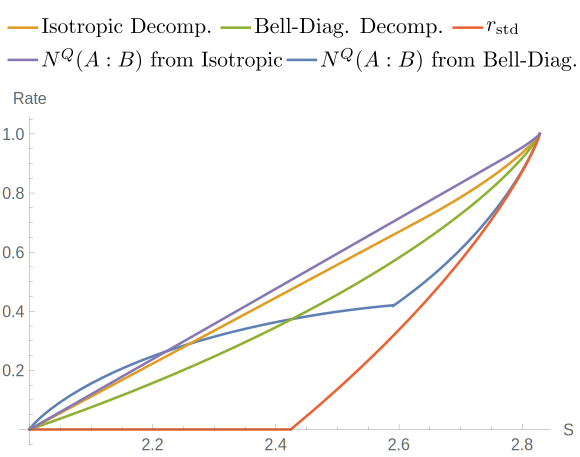
\includegraphics[width=\linewidth]{new_plot.pdf}
        \caption[Comparison of upper bounds.]{\label{fig:genubound} Upper bounds based on \Cref{eqn:genubound_state} for a specific CHSH-based implementation, with either Bell-diagonal states or isotropic states used in the decomposition. The bounds from quantum intrinsic nonlocality~\cite{DIQKD_Limits}~\cite[Appendix B]{RevisedPeres} are plotted for comparison. (Source:~\cite{CCSquashedEntangle})}
      \end{figure}

      For any arbitrary DIQKD protocol, an upper bound for a specific qqq state and measurement strategy is given by~\cite[Thm. 3]{CCSquashedEntangle}
      \begin{equation}\label{eqn:genubound_state}
        C^{\otimes}_{\sk}(\rho_{ABE}, \sM) \leq \inf_{\substack{q : \\ \rho = (1-q)\rho^{NL} + q\rho^L}} (1-q) \inf_{\substack{\sigma^{NL}, \sN : \\ \cP(\sigma^{NL}, \sN) \\ = \cP(\rho^{NL}, \sM) }} E_R(\sigma^{NL}) + q \inf_{\substack{\sigma^L, \sN : \\ \cP(\sigma^L, \sN) \\ = \cP(\rho^L, \sM) }} E_R(\sigma^L),
      \end{equation}
      where \(\cP(\rho^L, \sM) \in \Ls\) and \(\cP(\rho^{NL}, \sM) \not\in \Ls\). Essentially, we decompose the state into local and nonlocal parts (where states are classified as local or nonlocal based on the behaviour produced using the chosen measurement strategy), and compute the relative entropy of entanglement for each part, then minimise over the possible states, measurements and decompositions. Due to the device-independence of the distillation protocol, Eve is free to choose any states and measurements that would not be device-independently distinguishable from the expected states and measurements used in the device.

      We can actually tighten this bound by generalising it to a bound on behaviours alone, without specifying any state or measurement.
      \begin{equation}\label{eqn:genubound_behav}
        C^{\otimes}_{\sk}(p) \leq \inf_{\substack{q, \sigma^{L}, \sN^{L}, \sigma^{NL}, \sN^{NL} : \\ p = (1-q)\cP(\sigma^{L}, \sN^{L}) + q\cP(\sigma^{NL}, \sN^{NL})}} (1-q) E_R(\sigma^{NL}) + q E_R(\sigma^L).
      \end{equation}
      Clearly, any choice of \(\{q, \sigma^{L}, \sN^{L}, \sigma^{NL}, \sN^{NL}\}\) that minimises \Cref{eqn:genubound_state} is a valid choice in the minimisation in \Cref{eqn:genubound_behav}, but in the latter minimisation, \(\cP(\sigma^{L}, \sN^{L})\) and \(\cP(\sigma^{NL}, \sN^{NL})\) are not constrained to match the behaviour given by a certain \(\{\rho, \sM\}\), as long as the overall behaviour is the same---which is the only thing that can be device-independently certified. Therefore,
      \begin{equation}
         C^{\otimes}_{\sk}\left( \cP(\rho_{ABE}, \sM) \right) \leq C^{\otimes}_{\sk}(\rho_{ABE}, \sM).
      \end{equation}

      While highly general, both variants of this bound are extremely difficult to compute, because of the vast, unstructured search space and the nested optimisation, including the optimisation for the relative entropy of entanglement. The authors themselves computed this bound only for a specific choice of the measurements, and specific decompositions of specific states parametrised by CHSH values, as shown in \Cref{fig:genubound}. These are \emph{isotropic states} with
      \begin{equation}
        \rho^{I}(v) = (1-v)\ket{\Psi_+}\bra{\Psi_+} + \frac{v}{4}I
      \end{equation}
      and \(S = 2\sqrt{2}(1-v)\), and \emph{Bell diagonal states} with
      \begin{equation}
        \rho^{\Psi}(C) = \frac{1+C}{2}\ket{\Psi_+}\bra{\Psi_+} + \frac{1-C}{2}\ket{\Psi_-}\bra{\Psi_-}
      \end{equation}
      and \(S = 2\sqrt{C^2+1}\), where the \emph{Bell states} are
      \begin{equation}
        \ket{\Phi_{\pm}} = \frac{1}{\sqrt{2}}\left( \ket{00} \pm \ket{11} \right) \qquad \ket{\Psi_{\pm}} = \frac{1}{\sqrt{2}}\left( \ket{01} \pm \ket{10} \right).
      \end{equation}
      Fortunately, since all the optimisations are infima, any choice for the parameters is by definition an upper bound, and this bound can be used to evaluate the performance of a protocol on a given implementation.

      % Bell states can be converted between each other with local unitaries

      The \emph{quantum intrinsic nonlocality} is~\cite{DIQKD_Limits}
      \begin{equation}
        N^Q{(\crv{A}:\crv{B})}_p = \sup_{p_{\rm in}(x,y)} \inf_{\rho_{\crv{ABXY}E}} I{(\crv{A}:\crv{B}|\crv{XY}E)}_{\rho},
      \end{equation}
       \(N^Q{(\crv{A}:\crv{B})}_p\) is an upper bound on a wide range of protocols, including those with two-way error correction, but excluding those where the measurement settings are not revealed. \(N^Q\) was proposed and evaluated on isotropic states with fixed measurements in~\cite{DIQKD_Limits}. For evaluating a CHSH-based protocol, where only the CHSH value, and not the full behaviour, is used to decide whether or not to abort, this implementation is outperformed by \Cref{eqn:genubound_state} using either Bell-diagonal or isotropic decompositions, both of which are in turn outperformed by an estimate of \(N^Q\) using Bell-diagonal states in~\cite[Appendix B]{RevisedPeres} for \(S \gtrsim 2.525\).

      Unfortunately, these bounds are faithful, at least for the implementations considered. There is thus far only one (possibly) non-faithful upper bound that has been found for quantum adversaries~\cite{NotSufficient}. Interestingly, it uses classical information processing to carry out the attack, by proving the existence of a classical strategy for Eve to reduce the conditional mutual information of Alice and Bob to 0, for behaviours that can be obtained by arbtirarily many projective measurements of a class of quantum states. However, like \(N^Q\), it applies only to DIQKD protocols where Alice and Bob announce their choice of basis, leaving open the possibility that protocols that do not involve such announcements, such as~\cite{NonstandardProtocol}, may be able to achieve positive key rates, so this is not completely conclusive evidence that \(C_{\sk} = 0\) for these behaviours. However, it seems that the particular protocol in~\cite{NonstandardProtocol} has only been proved secure against individual attacks, and it might be interesting to see if it can be proved secure against collective attacks.

      \begin{question}
        What is the key rate of~\cite{NonstandardProtocol} secure against collective attacks?
      \end{question}

      Returning to the bound in~\cite{NotSufficient}, it is known that \emph{Werner states} with visibility \(v\)
      \begin{equation}
        \rho^{W}(v) = v{\ket{\Psi_-}\bra{\Psi_-}} + \frac{1-v}{4}I,
      \end{equation}
      cannot exhibit nonlocality for \(v < v_L \approx 0.6829\), but can do so for \(v \geq v_{NL} \approx 0.6964\). However, it is shown that for \(v < v_{\crit} \approx 0.7263 > v_{NL}\), any measurement strategy using projective measurements will produce correlations that can be expressed as a convex combination of behaviours that gives \(I(\crv{A}:\crv{B} \downarrow E) = 0\), implying that \(C_{\sk} = 0\) for all such correlations. Since \(v_{NL} < v_{\crit}\), this includes some correlations that exhibit nonlocality. The critical visibility can be increased even further for specific protocols. These behaviours, then, are prospective targets for revival. However, while we are able to specify some behaviours within this set, it is not clear what this set looks like in general. Characterising it might give more insight into how to go about reviving this region.

      \begin{question}
        Can we characterise the quantumly achievable behaviours from Werner states of a given visibility?
      \end{question}

      Many of these bounds were generalised and superseded using the \emph{classical-classical (cc) squashed entanglement} defined in~\cite{CCSquashedEntangle} as
      \begin{equation}
        E^{cc}_{sq}(\rho, \sM, p_{\rm in}(x,y)) = \sum_{xy} p_{\rm in}(x,y) \inf_{\cE_{x,y}} I{(\crv{A} : \crv{B}|E)}_{\cE_{x,y}(\psi^{\rho})},
      \end{equation}
      where \(\cE_{x,y}\) measures \(\psi^\sigma\), the purification of \({\sigma}\), using the POVMs in \(\sM\) corresponding to \(x\) and \(y\), while applying an arbitrary CPTP map to Eve's system. Notably, this function is convex in \(\rho\). This bound for states and measurements yields several different bounds for behaviours that generally improve on previous results. Denoting the key-generating inputs as \((\hat{x},\hat{y})\), the error rate in the key-generating basis as \(Q(p) = p(a\neq{b}|\hat{x}\hat{y})\) and the value of some function corresponding to the LHS of a Bell inequality as \(\hat{S}\), we have
      \begin{align}
        E^{cc,(\hat{x},\hat{y})}_{sq,par}(p) &= \inf_{\substack{\rho, \sM : \\ \hat{S}(p) = \hat{S}(\cP(\rho, \sM)) \\ Q(p) = Q(\cP(\rho, \sM)) }} E^{cc}_{sq}(\rho, \sM, \{p_{\rm in}(\hat{x},\hat{y})=1\}) \\
        E^{cc,(\hat{x},\hat{y})}_{sq,dev}(p) &= \inf_{\substack{\rho, \sM : \\ p = \cP(\rho, \sM)}} E^{cc}_{sq}(\rho, \sM, \{p_{\rm in}(\hat{x},\hat{y})=1\}) \\
        E^{cc}_{sq,dev}(p) &= \inf_{\substack{\rho, \sM : \\ p = \cP(\rho, \sM)}} E^{cc}_{sq}(\rho, \sM, p_{\rm in}(x,y)).
      \end{align}

      We define the \emph{lower convex envelope} \(\LCxE{\{f_i\}} = \tilde{f}\) of a set of functions \(\{f_i\}\) as
      \begin{equation}\label{eqn:LCxEdef}
        \tilde{f}(x) = \max\{ f(x) : \forall x, i : f(x) \leq f_i(x) \land f\text{ convex} \},
      \end{equation}
      and compare the bounds and their domains of validity in \Cref{tab:ccsqcomp}.

      \begin{table}
        \begin{tabular}{|p{\tableline{0.3}}|p{\tableline{0.7}}|}
          \hline
          \( E^{cc,(\hat{x},\hat{y})}_{sq,par} \leq \LCxE{\{I_{AL}, I_{FBJKL+}\}} \) & For any protocol that uses one key-generating basis and the statistics \(Q\) and \(\hat{S}\), if these statistics can be generated from Werner states with projective measurements, \(I_{AL}\) is an upper bound for intrinsic information computed in~\cite{RevisedPeres}, while \(I_{FBJKL+}\) is the non-faithful upper bound from~\cite{NotSufficient}. However, \(E^{cc,(\hat{x},\hat{y})}_{sq,par}\) is a convex upper bound for the key rate, and a lower bound for their lower convex envelope, which itself is a convex upper bound for the key rate. \\ \hline
          \( E^{cc,(\hat{x},\hat{y})}_{sq,dev} \leq I_{FBJKL+} \) & For any behaviour that can be generated from Werner states with projective measurements, and any protocol that broadcasts the input settings, \(I_{FBJKL+}\) is the non-faithful upper bound from~\cite{NotSufficient}. However, \(E^{cc,(\hat{x},\hat{y})}_{sq,par}\) is a convex upper bound for the key rate, and a lower bound for \(I_{FBJKL+}\). \\ \hline
        \end{tabular}
        \caption{\label{tab:ccsqcomp} Comparison between bounds from cc-squashed entanglement and earlier results.}
      \end{table}

      Once again, it is fortunate that all optimisations are infima, because this is a difficult optimisation to compute. Although it was applied to bound a specific set of protocols, it might be interesting to see if it could have more general applicability.

      \begin{question}
        What bounds on general protocols can we achieve using the cc-squashed entanglement?
      \end{question}

      \subsection{Lower Bounds from Asymmetric CHSH}

      Instead of using the CHSH inequality directly, it is possible to compute key rates in the standard protocol using asymmetric versions of the CHSH expression
      \begin{equation}
        S_{\alpha} \coloneqq \alpha\angleb{A_0 B_0} + \alpha\angleb{A_1 B_0} + \angleb{A_0 B_1} - \angleb{A_1 B_1}.
      \end{equation}
      This technique can then be combined with noisy preprocessing, where Alice replaces each bit of her key with a locally random bit with probability \(q\). The lower bound for \(H(\crv{A}|E)\), with \(s = S_{\alpha}\) from the test statistics, is
      \begin{equation} H(\crv{A}|E) \geq g_{q,\alpha}(s) = \begin{cases}
        g(s) & \text{ for } \abs{\alpha} \geq 1 \text{ or } s \geq s^* \\
        h_2(q) + g'(s^*)(\abs{s}-2) & \text{ otherwise},
      \end{cases}
    \end{equation}
    where
    \begin{equation}
      g_{q,\alpha}(s) = 1 + \phi\left(R_1\right) - \phi\left(R_2\right),
    \end{equation}
    with \(\phi(x) = h_2(1/2 + x/2)\) and
    \begin{equation} 
      R_1 = \sqrt{{(1-2q)}^2 + 4q(1-q)(s^2/4-\alpha^2)} \qquad R_2 = \sqrt{s^2/4-\alpha^2}
    \end{equation}
    and where \(s^*\) is the solution to
    \begin{equation}\label{eqn:sstar}
      h_2(q) + g'(s^*) (s^*-2) = g(s^*).
    \end{equation}

    For a function \(R(s)\) of \(s\), it can easily be verified that
    \begin{equation}
      \diff{\phi(R)}{s} = \frac{1}{2} \diff{R}{s} \log\frac{1-R}{1+R},
    \end{equation}
    and since
    \begin{equation} 
      R_1'(s) = \frac{qs(1-q)}{R_1} \qquad R_2'(s) = \frac{s}{4R_2},
    \end{equation}
    we have
    \begin{equation}\label{eqn:diffg}
      g_{q,\alpha}'(s) = \frac{qs(1-q)}{2R_1} \log\frac{1-R_1}{1+R_1} - \frac{s}{4R_2} \log\frac{1-R_2}{1+R_2}.
    \end{equation}

    The chief difficulty in evaluating this lower bound is optimising the values of \(\alpha\) and \(q\), since the value for \(s^*\) depends on them, but we do not have a closed form expression for it in terms of \(\alpha\) and \(q\). In order to sidestep this issue, we split the problem into three separate optimisations over three parameter regimes, add \(s^*\) as a variable, and enforce \Cref{eqn:diffg} as a constraint where necessary:
    \begin{enumerate}
      \item \(\abs{\alpha} \geq 1\): optimise with \(g_{q,\alpha}(s)\); no need for \(s^*\)
      \item \(\abs{\alpha} \leq 1\) and \(s \leq s^*\): optimise with \(h_2(q) + g'(s^*)(\abs{s}-2)\), constrain \(s^*\) with \Cref{eqn:diffg}
      \item \(\abs{\alpha} \leq 1\) and \(s \geq s^*\): optimise with \(g_{q,\alpha}(s)\), constrain \(s^*\) with \Cref{eqn:diffg}
    \end{enumerate}

    \subsection{Lower Bounds from Quasi-Relative Entropies}\label{sec:diqkd_qre}

    A recent approach to lower bounding the secret key uses semidefinite programming to directly compute lower bounds on \(H{(\crv{A}|E)}_{\rho}\), among all states \(\rho\) compatible with a given behaviour, by characterising the conditional entropy as a relative entropy
    \begin{equation}
      H{(\crv{A}|E)}_{\rho} = -D(\rho_{\crv{A}E}||I_\crv{A} \otimes \rho_{E}).
    \end{equation}
    Although it does not construct an explicit protocol or implementation, it is still a useful theoretical tool for identifying lower bounds.

    As the authors wanted to develop highly general tools that can be used to calculate a variety of quantities and that would work even for infinite-dimensional cases, they made use of the operator algebra approach to quantum mechanics and spectral theory, which are generally not covered in undergraduate treatments of quantum mechanics and quantum information. Some of these technicalities have been reviewed in \Cref{sec:qretech}, but for this section, we write the expressions in finite-dimensional form, where all spectra are discrete.

    The set of \emph{bounded operators} \(\mathcal{B}(\Hs)\) on the Hilbert space \(\Hs\) is the subset of \(\mathcal{L}(\Hs)\), the set of all linear operators on \(\Hs\), such that the \emph{operator norm} of \(X \in \mathcal{L}(\Hs)\)
      \[ \norm{X} \coloneqq \sup_{\psi \in \Hs \setminus \{0\}} \frac{\norm{X\psi}}{\norm{\psi}} \]
      is finite. An operator \(X \in \mathcal{B}(\Hs)\) is \emph{trace-class} if, for the positive, self-adjoint operator \(\sqrt{X^{\dagger}X}\),
      \[ \Tr\left[ \sqrt{X^{\dagger}X} \right] = \sum_{i} \angleb{e_i, Xe_i} \leq +\infty \]
      for any orthonormal basis \(\{e_j\}\) for \(\Hs\)~\cite{HallQuantumForMath}. 

      The natural logarithm has the integral representation
      \begin{equation}
        \ln\left(\frac{x}{y}\right) = -\int_{0}^{1} \frac{x-y}{t(x-y) + y} \dif{t}.
      \end{equation}
      Therefore, we can write the relative entropy as
      \begin{align}
        D(\rho||\sigma) &= \frac{1}{\ln 2} \Tr\left[\rho \left(\ln\rho - \ln\sigma\right) \right] \\
                        &= \frac{1}{\ln 2} \Tr\left[ \sum_{x,y} y \ln\left(\frac{y}{x}\right) \Pi^{(x)}_{\sigma} \Pi^{(y)}_{\rho}  \right]\label{eqn:finitedim_relent} \\ 
                        &= -\frac{1}{\ln 2} \Tr\left[ \sum_{x,y} y \int_{0}^{1} \frac{x-y}{t(x-y)+y} \Pi^{(x)}_{\sigma} \Pi^{(y)}_{\rho} \dif{t} \right],
      \end{align}
      where \(x\) and \(y\) are eigenvalues of \(\sigma\) and \(\rho\), and \(\Pi^{(x)}_{\sigma}\) and \(\Pi^{(y)}_{\rho}\) are their respective eigenprojectors.

      This integral can be approximated by the \(m\)-point \emph{Gauss-Radau quadrature}, such that \(t_m = 1\), \(w_m = 1/m^2\), and
      \begin{equation}
        \int_{0}^{1} g(t) \dif{t} \geq \sum_{i=1}^m w_i g(t_i).
      \end{equation}
      The \(t_i \in \ocintv{0}{1}\) are referred to as \emph{nodes}, while the \(w_i > 0\) are \emph{weights}. These nodes and weights are special in that equality is achieved if \(g(t)\) is a polynomial of degree less than \(2m-2\).

      The key insight of this method is in observing that this sum can be commuted with the sum over the eigenvalues to obtain
      \begin{equation}
        D(\rho||\sigma) = - \sum_{i=1}^{m} \frac{w_i}{\ln 2} \underbrace{\Tr\left[ \sum_{x,y} y \frac{x-y}{t_i(x-y)+y} \Pi^{(x)}_{\sigma} \Pi^{(y)}_{\rho} \right]}_{\eqqcolon D_{F_{t_i}}(\rho||\sigma)},\label{eqn:re_from_qre}
      \end{equation}
      and that the \emph{quasi-relative entropy} \(D_{F_{t}}(\rho||\sigma)\) can be characterised variationally as
      \begin{equation}
        D_{F_{t}}(\rho||\sigma) = \frac{1}{t} \inf_Z \Tr\left[ \rho + \rho(Z + Z^{\dagger}) + (1-t)\rho{}Z^{\dagger}Z + t\sigma{}ZZ^{\dagger}. \right]\label{eqn:qre_var}
      \end{equation}
      This variational expression is of the form \(\Tr[\rho P]\), where \(P\) is a polynomial of operators. As will be seen later, optimisations of this form can be efficiently approximated (with some technical caveats).

      Putting all these results together, and with some additional effort to prove convergence and boundedness of the operators, we have, for trace-class operators \(\rho, \sigma \in \mathcal{L}(\Hs)\), where \(\rho \leq \lambda\sigma\) for some \(\lambda \in \R^+\),
      \begin{equation}
        D(\rho||\sigma) \leq c_m - \sum_{i=1}^{m-1} \frac{w_i}{t_i \ln 2} \inf_{\substack{Z \in \sB(\Hs) : \\ \norm{Z} \leq \alpha_i}} \Tr\left[\rho\left(Z + Z^{\dagger}\right)\right] + (1-t_i)\Tr\left[\rho\left(Z^{\dagger}Z\right)\right] + t_i\Tr\left[\sigma\left(ZZ^{\dagger}\right)\right],
      \end{equation}
      where
      \begin{equation}
        c_m = \frac{1}{m^2} \frac{\lambda \Tr[\rho]}{\ln 2} - \sum_{i=1}^m \frac{w_i \Tr[\rho]}{t_i \ln 2} \qquad \alpha_i = \frac{3}{2} \max\left\{\frac{1}{t_i}, \frac{\lambda}{1-t_i}\right\}.
      \end{equation}
      This inequality converges as \(m \to \infty\).

      For DIQKD protocols that use a specific input, say \(x^{\star}\), to generate the key, we can apply this analysis to bound the relevant conditional entropy \(H{(\crv{A}|E, \crv{X}=x^{\star})}_{\rho}\) by observing that
      \begin{align*}
        H{(\crv{A}|E)}_{\rho} &= \log d_A - D(\rho_{\crv{A}E}||I_{\crv{A}}\otimes\rho_{E} / d_A) \\
                              &= \log d_A - \Tr\left[\rho_{\crv{A}E}(\log(\rho_{\crv{A}E}) - \log(I_{\crv{A}}\otimes\rho_{E} / d_A))\right] \\
                              &= \log d_A - \Tr\left[\rho_{\crv{A}E}(\log(\rho_{\crv{A}E}) - \log(I_{\crv{A}}\otimes\rho_{E}) + \log d_A)\right] \\
                              &= -\Tr\left[\rho_{\crv{A}E}(\log(\rho_{\crv{A}E}) - \log(I_{\crv{A}}\otimes\rho_{E}))\right] = -D(\rho_{\crv{A}E}||I_{\crv{A}}\otimes\rho_{E}),
      \end{align*}
      where \(d_A\) is the dimension of Alice's system and \(I_A/d_A\) is the state representing a uniform distribution for Alice's system.

      Then, with \(r\) arbitary linear constraints on the behaviour, indexed by \(j\)
      \[ \sum_{abxy} c^{(j)}_{abxy} p(ab|xy) \geq v_j, \]
      and recalling that
      \[ p(ab|xy) = \Tr\left[\rho_{A B E} \left(M_{a|x} \otimes N_{b|y} \otimes I_{E}\right) \right], \]
      we can obtain lower bound:
      \begin{equation}
        H{(\crv{A}|E, \crv{X}=x^{\star})}_{\rho} \geq c_m + C_m(\rho),
      \end{equation}
      where \(C_m(\rho)\) is given by
      \begin{equation}
        \begin{aligned}[c]
          \inf & \sum_{i=1}^{m-1} \frac{w_i}{t_i \ln 2} \sum_a \Tr\left[ 
            \rho_{A B E} \left(
            \begin{gathered}
            M_{a|x^{\star}} \otimes I_{B} \otimes \left[ Z_{a,i} + Z_{a,i}^{\dagger} + (1-t_i)  Z_{a,i}^{\dagger}Z_{a,i} \right] \\
            + t_i \left( I_{A B} \otimes Z_{a,i}Z_{a,i}^{\dagger}\right) 
            \end{gathered}
            \right)
          \right] \\
          \text{s.t.} & \begin{aligned}[t] 
            & \sum_{abxy} c^{(j)}_{abxy} \Tr\left[\rho_{A B E} \left(M_{a|x} \otimes N_{b|y} \otimes I_{E}\right) \right] \geq v_j & & \forall 1 \leq j \leq r \\
            & \sum_{a} M_{a|x} = I_{A}, \sum_{b} N_{b|y} = I_{B} & & \forall x, y \\
            & M_{a|x} \geq 0, N_{b|y} \geq 0 & & \forall a, b, x, y \\
            & \norm{Z_{a,i}} \leq \alpha_i & & \forall a, i \in \dintv{1}{m-1} \\
            & M_{a|x} \in \sB(A), N_{b|y} \in \sB(B), Z_{a,i} \in \sB(E) & & \forall a, b, x, y, i \\
            & \rho_{A B E} \text{ is a valid state} & &
          \end{aligned}
        \end{aligned}
      \end{equation}

      We can use Naimark's dilation theorem to construct a state \(\tilde{\rho}\) and projective measurement operators\footnote{Projective in the sense that \(\tilde{M}_{a|x}\tilde{M}_{a'|x} = \delta_{a,a'}\tilde{M}_{a|x}\), with the analogous relation for Bob.} \(\{\tilde{M}_{a|x}, \tilde{N}_{b|y}\}\) on a Hilbert space \(\Hs\), such that \(\Tr\left[\tilde{\rho}\tilde{M}_{a|x}\right] = \Tr\left[\rho M_{a|x}\right]\) and  \(\Tr\left[\tilde{\rho}\tilde{N}_{b|y}\right] = \Tr\left[\rho N_{b|y}\right]\): that is, the behaviour remains the same. These can be mapped to the original behaviour and states via local isometries. We can further assume that the state is pure, that is, \(\tilde{\rho} = {\ket{\psi}\bra{\psi}}_{\Hs}\), which can only help Eve (due to the data-processing inequality).

      Additionally, instead of enforcing the tensor product explicitly, we can enforce that the operators \(Z_{a,i}\) commute with all \(\tilde{M}_{a|x}\) and \(\tilde{N}_{b|y}\), which in turn commute with each other.\footnote{This is equivalent to enforcing the tensor product structure in finite dimensions, but in infinite dimensions it may lead to a looser bound.} Therefore, we can replace all instances of \(\Tr\left[\rho S\right]\) in our objective function with \(\braket{\psi|\tilde{S}|\psi}\) for all monomials \(S\) (individual operators and products of operators), where \(\tilde{S}\) is the monomial with all measurements replaced by their projective versions on \(\Hs\). 

      These inner products can then be seen as elements of a Gram matrix for the vectors \(\{\ket{\psi}, \tilde{S}\ket{\psi}\}\), which must be positive semidefinite. In order to constrain \(\ket{\psi}\) to be a valid quantum state, we introduce more vectors of the form \(\prod M\ket{\psi}\) to our Gram matrix, where \(M \in \{\tilde{M}_{a|x}, \tilde{N}_{b|y}\}\). If these are valid states and measurements, the Gram matrix should still be positive semidefinite, even if we include vectors that result from an arbitrarily long sequence of measurement operators applied to \(\ket{\psi}\). This is the \emph{NPA hierarchy}, which is a converging hierarchy of approximations to the set of quantumly realisable states and measurements.\footnote{Recent results imply that we only have convergence in the finite-dimensional case; in infinite dimensions, the set of states and measurements converged to is strictly larger than that allowed by quantum theory.} Higher levels of the hierarchy involve monomials consisting of longer chains of measurement operators. The final expression for \(C_m\) then becomes
      \begin{equation}
        \begin{aligned}[c]
          \inf & \sum_{i=1}^{m-1} \frac{w_i}{t_i \ln 2} \sum_a \angleb{\psi\left|
          \tilde{M}_{a|x^{\star}} \left( Z_{a,i} + Z_{a,i}^{\dagger} + (1-t_i)  Z_{a,i}^{\dagger}Z_{a,i}\right) + t_i Z_{a,i}Z_{a,i}^{\dagger} \right|\psi} \\
            \text{s.t.} & \begin{aligned}[t] 
          & \sum_{abxy} c^{(j)}_{abxy} \angleb{\psi\left| \tilde{M}_{a|x} \tilde{N}_{b|y} \right|\psi} \geq v_j & & \forall 1 \leq j \leq r \\
          & \sum_{a} \tilde{M}_{a|x} = I_{A}, \sum_{b} \tilde{N}_{b|y} = I_{B} & & \forall x, y \\
          & \tilde{M}_{a|x} \geq 0, \tilde{N}_{b|y} \geq 0 & & \forall a, b, x, y \\
          & Z_{a,i} Z_{a,i}^{\dagger} \leq \alpha_i & & \forall a, i \in \dintv{1}{m-1} \\
          & Z_{a,i}^{\dagger} Z_{a,i} \leq \alpha_i & & \forall a, i \in \dintv{1}{m-1} \\
          & \tilde{M}_{a|x}, \tilde{N}_{b|y}, Z_{a,i} \in \sB(\Hs) & & \forall a, b, x, y, i \\
          & [\tilde{M}_{a|x}, \tilde{N}_{b|y}] = [\tilde{M}_{a|x}, Z_{b,i}] = [\tilde{N}_{b|y}, Z_{a,i}] = 0 & & \forall a, b, x, y, i \\
          & [\tilde{M}_{a|x}, Z_{b,i}^{\dagger}] = [\tilde{N}_{b|y}, Z_{a,i}^{\dagger}] = 0 & & \forall a, b, x, y, i \\
          & \ket{\psi} \text{ is a valid state} & & \\
            \end{aligned}
        \end{aligned}
      \end{equation}

      A few other simplifications are possible, which are discussed and implemented in~\cite{BFF_QRE}:
      \begin{enumerate}
        \item From the normalisation of the measurements, we have that \(\tilde{M}_{o_A|x} = I - \sum_{a < o_A} \tilde{M}_{a|x}\). This allows us to eliminate one measurement operator for each value of \(x\), with the analogous simplification for Bob.
        \item We need only consider inequalities that involve the operators in the objective function, since the other operators can be set to any value without changing the value of the objective function. For a protocol that depends only on the specific input \(x^{\star}\), this means that we need only consider inequalities that involve \(M_{a|x^{\star}}\). Therefore, we need only consider the operators appearing in those inequalities.
        \item We can commute the infimum with the sum. That is, we use the objective function
          \begin{equation} 
            \sum_{i=1}^{m-1} \inf \frac{w_i}{t_i \ln 2} \sum_a \angleb{\psi\left|
          \tilde{M}_{a|x^{\star}} \left( Z_{a,i} + Z_{a,i}^{\dagger} + (1-t_i)  Z_{a,i}^{\dagger}Z_{a,i}\right) + t_i Z_{a,i}Z_{a,i}^{\dagger} \right|\psi},
          \end{equation}
          solving \(m-1\) SDPs in sequence. This avoids an optimisation with \((m-1)o_A\) operators \(Z_{a,i}\), which would result in a vastly larger problem that will take much longer to solve. Since the variables in each SDP can be now be varied independently, this can only decrease the infimum computed, thereby decreasing the lower bound on the entropy, but still providing a valid lower bound on the entropy.
        \item The inequality constraints on the operators can be removed in order to speed up the optimisation. Once again, this decreases the value of the achievable infimum, giving a looser but still valid lower bound.
      \end{enumerate}

      Given the generality of these techniques, one could wonder whether any upper bounds can be computed in this fashion as well. This might help alleviate the optimisation difficulties discussed previously. The quadrature would need to be changed to be an upper bound, rather than a lower bound.
      \begin{question}
        Can any known upper bounds be formulated as quasi-relative entropies and approximated with this method?
      \end{question}

    \section{Preliminary Results}\label{sec:preres}

    Our preliminary results found a revival of the standard protocol key rate for states that are generated according to a simple experimental model. We will be using it to illustrate the relevant issues and directions we wish to pursue in our analysis. In this model, we denote the density matrix of Alice's and Bob's quantum state as \(\rho_{AB}\) and observables as \(\tilde{A}_x\) and \(\tilde{B}_y\) for a perfect experimental setup, and let the dimensions of the Hilbert spaces of systems \(A\) and \(B\) be \(d_A\) and \(d_B\) respectively.

    We now model some possible experimental flaws. If our source of quantum states produces one state per time bin, then \(n_c\) is the probability that a state is not produced during a given time bin (where we assume this process to be i.i.d.). Further, Alice and Bob's detectors have efficiencies \(\eta_A\) and \(\eta_B\) respectively, which are the probabilities for them to detect a state given that one is produced. If nothing is detected, either due to no signal being produced or due to detector inefficiency, we assign the \(-1\) outcome. The detector failure events are independent, but if no signal is produced, both Alice and Bob will receive no signal. We can then express the new states and observables as follows:
    \begin{align*}
      A_x &= (1-\eta_A)\tilde{A}_x - \eta_A I_A \\
      B_y &= (1-\eta_B)\tilde{B}_y - \eta_B I_B \\
      \rho_{{A_x}{B_y}} &= (1-n_c)\tilde{\rho}_{{A_x}{B_y}} + \frac{n_c}{d^{(0)}_{A_x} d^{(0)}_{B_y}} \left( \Pi_{A_x}^{(0)} \otimes \Pi_{B_y}^{(0)} \right),
    \end{align*}
    where \(I_A\) is the identity operator on Alice's Hilbert space, and \(d^{(0)}_{A_x}\) is the dimension of the subspace that \(\Pi_{A_x}^{(0)}\) projects onto, with the analogous definitions holding for \(B\).

    The marginals and correlators, then, are as follows:
    \begin{align*}
      \angleb{A_x} &= -n_c + (1-n_c)(\eta_A\angleb{\tilde{A}_x} - (1-\eta_A)) \\
      \angleb{B_y} &= -n_c + (1-n_c)(\eta_B\angleb{\tilde{B}_y} - (1-\eta_B)) \\
      \angleb{A_x B_y} &= \begin{aligned}[c]
      & n_c + (1-n_c)(\eta_A\eta_B\angleb{\tilde{A}_x\tilde{B}_y} - \eta_A(1-\eta_B)\angleb{\tilde{A}_x} \\
      & -\eta_B(1-\eta_A)\angleb{\tilde{B}_y} + (1-\eta_A\eta_B) )
      \end{aligned}
      \end{align*}

      For our purposes, we fix \(\eta_A = \eta_B = \eta\). We want to study the variation of the key rate with the variation of these parameters. Since \(S\) is a linear combination of the correlators, we only need to compute the variation of the correlators with \(\eta\) and \(n_c\). We connect this to the key rate by studying the variation of \(H_S(\crv{A}|E)\) with \(S\).
      \begin{align*}
        \diffp{}{{n_c}} \angleb{A_x B_y} &= \eta \left( \left(1-\eta\right) \left(\langle\tilde{A}_x\rangle + \langle\tilde{B}_y\rangle\right) - \eta \langle\tilde{A}_x\tilde{B}_y\rangle + \left(2 - \eta\right) \right) \\
        \diffp{}{{\eta}} \angleb{A_x B_y} &= \left(1 - n_{c}\right) \left( \left(1-2\eta\right) \left(\langle\tilde{A}_x\rangle+\langle\tilde{B}_y\rangle\right) - 2\eta \langle\tilde{A}_x\tilde{B}_y\rangle + (2-2\eta) \right) \\
        \diffp{}{S} H_S(\crv{A}|E) &= \frac{S}{4\sqrt{S^2-4}} \log_2 \left[ \frac{\sqrt{S^2-4}-2}{\sqrt{S^2-4}+2} \right].
      \end{align*}

    \begin{figure}
      \centering
      \includegraphics[width=\linewidth]{exptplt.pdf}
      \caption{\label{fig:exptplt} Minimum \(\eta\) required for \(r_{\std} > 0\), given \(n_c\).}
    \end{figure}

      Consider the following simple wiring, the \emph{N-AND wiring}, where we broadcast the same inputs \(x\) and \(y\) to \(N\) boxes on each side, and drive an AND gate with all the outputs. Clearly, this can only increase the correlations between Alice and Bob, since \(a \neq b\) only if all \(N\) boxes return different outputs to Alice and Bob. However, this means that if Eve knows that any of the boxes produced 0, she can conclude that the overall output is 0, increasing her correlation with Alice. If the increase in \(H(\crv{A}|\crv{B})\) can make up for the decrease in \(H(\crv{A}|E)\), then this wiring improves the key rate.

      For \(N\) boxes, the correlators and marginals become
      \begin{gather}
        \angleb{A_x B_y}_{N} = 1 - \frac{{(1-\angleb{B_y})}^N + {(1-\angleb{A_x})}^N}{2^{N-1}} + \frac{1}{4^{N-1}} {(1-\angleb{A_x} - \angleb{B_y} + \angleb{A_x B_y})}^{N} \\
        \angleb{A_x}_{N} = 1 - 2 {\left(\frac{1-\angleb{A_x}}{2}\right)}^N \qquad \angleb{B_y}_{N} = 1 - 2 {\left(\frac{1-\angleb{B_y}}{2}\right)}^N,
      \end{gather}
      and we denote the resultant behaviour as \(p_N\).

      Using the standard protocol key rate, we are able to find \emph{revival} in certain parameter regimes: behaviours with \(r_{\std}(p) = 0\), but which have \(r_{\std}(p_N) > 0\), as shown in \Cref{fig:exptplt}. However, since wiring no longer treats the individual rounds as i.i.d., it should not be used as part of a protocol for the purpose of computing \(C_{\sk}\). Therefore, it is possible that \(C_{\sk}(p_N) > C_{\sk}(p)\). However, it might just be that \(r_{\std}(p) < C_{\sk}(p)\), and that the wiring does not improve the secret key capacity. We can now state one of the aims of our research more precisely:
      \begin{funqn}\label{fqn:wircap}
        Can wiring increase the secret key capacity of a behaviour?
      \end{funqn}

      From a theoretical standpoint, answering this question would develop our currently limited understanding of the nature of the secret key capacity, and practically, the use of such wirings would be an easily-implemented technique that can squeeze secrecy out of a poorly-functioning system. ``Super-activation'' of nonlocality is known to exist for joint quantum operations (e.g.\ two quantum states that do not exhibit nonlocality individually can jointly exhibit it), so there is some hope that similar behaviour might be observed here.

      TODO write out how NL activation can be done in more detail

      \section{Local Wirings}\label{sec:locwir}

      Before proceeding with our analysis, we must define what we mean by ``wirings''. In other words, we must define our \emph{resource theory}. Our approach is based on that of~\cite{BellResourceTheory}, which also reviews the following preliminary material. Taking inspiration from entanglement theory, which studies entanglement as a resource, a more general resource theory defines a set of \emph{free resources} and a set of \emph{free actions}, and studies how the resources in the theory can be converted between each other using only those free actions and free resources. If it is possible to convert a resource \(R_1\) into a resource \(R_2\), we write \(R_1 \leadsto R_2\), and we write \(R \not\leadsto S\) otherwise. This relation defines a \emph{pre-order} for the resource theory: given any two resources \(R_1\) and \(R_2\), one of the following statements must hold
      \begin{itemize}
        \item \(R_1\) is \emph{strictly below} \(R_2\): \(R_1 \not\leadsto R_2\) and \(R_2 \leadsto R_1\)
        \item \(R_1\) is \emph{strictly above} \(R_2\): \(R_1 \leadsto R_2\) and \(R_2 \not\leadsto R_1\)
        \item \(R_1\) is \emph{incomparable to} \(R_2\): \(R_1 \not\leadsto R_2\) and \(R_2 \not\leadsto R_1\)
        \item \(R_1\) is \emph{equivalent to} \(R_2\): \(R_1 \leadsto R_2\) and \(R_2 \leadsto R_1\)
      \end{itemize}

      While there has been a recent resurgence of interest in developing resource theories of nonlocality and other unusual quantum phenomena, much of the recent work is too abstract and general to be directly applied by us~\cite{Monotones, TypeIndepLOSR}, or focuses only on \emph{single-copy conversions} using \emph{local operations and shared randomness} (LOSR) as the set of free actions~\cite{BellResourceTheory, TraceDistNL, NLMeas}, instead of the multiple-copy conversions that wirings perform (with a notable exception discussed in \Cref{sec:nlmono_maxcorr}).

      LOSR actions transform \(p(a_0 b_0|x_0 y_0) \mapsto p'(ab|xy)\) using a conditional distribution \(\chi\):
      \begin{equation}
        p'(ab|xy) = \sum_{abxy} \chi(abx_0y_0|a_0b_0xy) p(a_0b_0|x_0y_0)
      \end{equation}
      that satisfies
      \begin{equation}
        \begin{aligned}[c]
        \chi(abx_0y_0|a_0b_0xy) = \sum_{\lambda} \chi_A(ax_0|a_0x\lambda) \chi_B(by_0|b_0y\lambda) p_{\Lambda}(\lambda),
        \end{aligned}
      \end{equation}
      where \(p_{\Lambda}\) is the distribution of the shared randomness, and \(\chi\) can be interpreted as a conditional probability within \(\Ls\), with outputs \((a, x_0)\) and \((b, y_0)\), and inputs \((a_0, x)\) and \((b_0, y)\). \(\chi_A\) and \(\chi_B\) must also satisfy the \emph{no-retrocausation} conditions:
      \begin{align}
        \chi_A(ax_0|a_0x\lambda) &= \chi_A(ax_0|x\lambda) \\
        \chi_B(by_0|b_0y\lambda) &= \chi_B(by_0|y\lambda).
      \end{align}
      In words, the value of \(x_0\) or \(y_0\) cannot depend on the value of \(a_0\) or \(b_0\), respectively, since the latter depend on the former.

      In this cryptographic scenario, it might be interesting to ask if there is any benefit to be gained from using \emph{private} shared randomness, unknown to Eve. 

      % TODO discuss this when talking about key rates

      However, if they have \(h\) bits of pre-shared randomness, since they are performing classical data processing, this can only increase Eve's entropy by at most \(h\), which can already be achieved by simply using the shared randomness as part of their secret key.

      Operationally, \(h\) bits of randomness will lead to \(2^h\) possible different behaviours.

      TODO can private correlation of the inputs improve Alice and Bob's entropy? Or does input correlation decrease entropy?

      TODO distinguish between: Eve knowing no inputs, Eve knowing overall inputs only, Eve knowing physical inputs only?, and Eve knowing both inputs.

      Private shared randomness does not help in deciding the overall outputs, since \(h\) bits of randomness will simply produce \(2^h\) different possibilities for the keys, which we would also obtain by using the private shared randomness as a key. FIXME is this correct?

      TODO maybe junk this section: no reason for this argument since we are considering shared randomness. Maybe argue, based on random basis paper approach, that private randomness forces Eve to not be able to tailor her attacks? Or is that irrelevant here?

      However, since our wirings combine multiple boxes, their effect cannot be expressed in this form. Nonetheless, we can straightforwardly generalise the expressions for LOSR operations, for \(c\) boxes wired together, as:
      \begin{gather}
        p'(ab|xy) = \sum_{\cvec{a}^c\cvec{b}^c\cvec{x}^c\cvec{y}^c} \chi(ab\cvec{x}^c\cvec{y}^c|\cvec{a}^c\cvec{b}^cxy) p(\cvec{a}^c\cvec{b}^c|\cvec{x}^c\cvec{y}^c)\label{eqn:wiringprobdef} \\
        \chi(ab\cvec{x}^c\cvec{y}^c|\cvec{a}^c\cvec{b}^cxy) = \sum_{\lambda} \chi_A(a\cvec{x}^c|\cvec{a}^cx \lambda) \chi_B(b\cvec{y}^c|\cvec{b}^cy \lambda) p_{\Lambda}(\lambda)\label{eqn:wiringfndef}
      \end{gather}
      where \(\cvec{a}^c = {(a_1, a_2, \ldots, a_c)}^{\rm T}\) is the vector of all the outputs from Alice's boxes that are wired together, with analogous definitions for \(\cvec{b}^c\), \(\cvec{x}^c\) and \(\cvec{y}^c\). In this context, we refer to \(\chi\) as the \emph{joint wiring function}. The set of no-retrocausation conditions is more complex, since the later boxes can depend on the output of the earlier boxes. If Alice and Bob interact with their boxes in increasing order of the index \(j\), we have:
      \begin{equation}
        \begin{aligned}[c]
        \chi_A(a\cvec{x}^j|\cvec{a}^cx\lambda) &= \chi_A(a\cvec{x}^j|\cvec{a}^{j-1}x\lambda),\,\forall j \in \dintv{1}{c} \\
        \chi_B(b\cvec{y}^j|\cvec{b}^cy\lambda) &= \chi_B(b\cvec{y}^j|\cvec{b}^{j-1}y\lambda),\,\forall j \in \dintv{1}{c},
        \end{aligned}\label{eqn:wiringnoretro}
      \end{equation}
      which we refer to as the \emph{marginal wiring functions}. If we focus only on \(j = c\), we can see these distributions as elements of \(\Ls\), with outputs \((a, \cvec{x}^c)\) and \((b, \cvec{y}^c)\), and inputs \((\cvec{a}^{c-1}, x)\) and \((\cvec{b}^{c-1}, y)\). These conditions will hopefully simplify the space of wirings, since without the conditions, we would have to processs \({(o_A i_A^c)}^{i_A^c o_A} {(o_B i_B^c)}^{i_B^c o_B}\) possible wirings (\(\approx \num{5.12e18}\) for the QKD setting). We will shortly turn our attention to characterising this space, but first briefly remark that, while the definitions and discussion thus far focus on the bipartite case, they generalise readily to the \(n\)-partite case, although we will not treat this case in detail here.

      \subsection{Wirings as Functions}

      Physically, a probabilistic wiring must actually execute some deterministic wiring, and its joint wiring function is then a probability distribution over the deterministic joint wiring functions, of which there are finitely many. This is the intuition behind the proof of Fine's theorem presented in~\cite{BellNonlocality}, which can be straightforwardly adapted to this polytope. Loosely speaking, given if there exists a decomposition of the behaviour into behaviours that obey the no-retrocausation conditions, these latter behaviours can be converted into deterministic behaviours obeying the conditions by offloading the indeterminism into an auxiliary random variable, and redefining \(\lambda\) to incorporate this auxliary variable.

      Therefore, to determine the polytope of joint wiring functions, we can use the same approach as is typically used for \(\Ls\), where deterministic operations are taken as the vertices of the polytope, and the facet-defining inequalities derived from there using a facet-enumeration algorithm. In order to avoid the computational effort of simply enumerating all possible local deterministic behaviours and pruning them by removing those that violate the no-retrocausation conditions, we wish to explore the structure of these wirings, so that we can minimise the generation of wirings that will eventually be pruned. Indeed, this analysis reveals significant redundancies in the wirings that would be generated naively, with many of them corresponding to the same action on the behaviours. Removing them at an early stage rather than generating and then dealing with them will increase the scalability of our methods.

      In order to illustrate one of the redundancies that emerges from the naive approach, we use a different, more operational description for deterministic wirings. Focusing on Alice's marginal wiring functions, we can decompose her marginal wiring function using Bayes' rule as
      \begin{align}
        \chi_A(a\cvec{x}^c|\cvec{a}^cx\lambda) &= \chi_A(a|\cvec{x}^c\cvec{a}^cx\lambda) \chi_A(\cvec{x}^{c}|\cvec{a}^cx\lambda) \\
        &= \chi_A(a|\cvec{x}^c\cvec{a}^cx\lambda) \chi_A(x_c|\cvec{x}^{c-1}\cvec{a}^cx\lambda) \chi_A(\cvec{x}^{c-1}|\cvec{a}^cx\lambda) \\
        &= \chi_A(a|\cvec{x}^c\cvec{a}^cx\lambda) \prod_{j=1}^c \chi_A(x_j|\cvec{x}^{j-1}\cvec{a}^cx\lambda) \\
        &= \chi_A(a|\cvec{x}^c\cvec{a}^{c}x\lambda) \prod_{j=1}^c \chi_A(x_j|\cvec{x}^{j-1}\cvec{a}^{j-1}x\lambda),
      \end{align}
      where in the last line we have used the no-retrocausation condition. For deterministic wirings, we can consider her inputs \(\cvec{x}^c\) to her boxes as being computed by a sequence of \(c\) deterministic functions with range \(\dintv{1}{i_A}\):
      \begin{equation} x_j = W^{(j)}_{A,\lambda}(\cvec{x}^{j-1}, \cvec{a}^{j-1}, x),\,j \in \dintv{1}{c} \end{equation}
      and a final output function with range \(\dintv{1}{o_A}\):
      \begin{equation} a = W_{A,\lambda}(\cvec{x}^{c}, \cvec{a}^{c}, x). \end{equation}
      We refer to each function \(W_{A,\lambda}\) as a \emph{marginal wiring map}. The corresponding marginal wiring function \(\chi_A\) is then
      \begin{equation}
        \chi_A(a\cvec{x}^c|\cvec{a}^cx\lambda) = \indic{a = W_{A,\lambda}(\cvec{x}^{c}, \cvec{a}^{c}, x)} \prod_{j=1}^c \indic{x_j = W^{(j)}_{A,\lambda}(\cvec{x}^{j-1}, \cvec{a}^{j-1}, x)}.
      \end{equation}
      The analogous definitions for Bob hold with the appropriate changes of labels \(A \mapsto B\), \(x \mapsto y\), \(a \mapsto b\). Probabilistic wirings can then be described as convex combinations of such deterministic wirings.

      We refer to the discrete set of deterministic marginal wiring functions that obey these relations as \(\sW_D\), and the polytope generated by them as vertices as \(\sW\). \(\sW^n\) is then the convex polytope with vertices \(\sW_D^n = \underbrace{\sW_D \times \sW_D \times \cdots \times \sW_D}_{n\text{ times}}\). We also define \(\sWB(p)\) as the set of behaviours generated by applying \(\sW^n\) to an \(n\)-partite behaviour \(p\) using \Cref{eqn:wiringprobdef}. In order to reduce ambiguity, we refer to wiring maps as mapping a \emph{source} to a \emph{target}, reserving ``input'' and ``output'' to describe the inputs and outputs of boxes.

      Using our classification for \(\sW_D\), simple combinatorics gives us \(i_A^{j} o_A^{j-1}\) possible sources for \(W^{(j)}_{A,\lambda}\). However, since the wiring is deterministic, \(x_j\) is completely fixed by \(\cvec{x}^{j-1}\), \(\cvec{a}^{j-1}\) and \(x\). Therefore, when considering each map as part of the overall wiring, the only free choice in the source is \(x\), and so there are only \(i_A o_A^{j-1}\) valid sources.

      \begin{table}
        \begin{minipage}{0.5\linewidth}
          \begin{center}
            \begin{tabular}{|r|cc|} \hline
              \diagbox{\(x x_1\)}{\(a_1\)} & 0 & 1 \\ \hline
              00 & 1 & 0 \\
              01 & X & X \\
              11 & 1 & 1 \\
              10 & X & X \\ \hline
            \end{tabular}
          \end{center}
        \end{minipage}
        \begin{minipage}{0.5\linewidth}
          \begin{center}
            \begin{tabular}{|r|cccc|} \hline
              \diagbox{\(x x_1 x_2\)}{\(a_1 a_2\)} & 00 & 01 & 11 & 10 \\ \hline
              000 & X & X & 1 & 0 \\
              001 & 0 & 0 & X & X \\
              011 & X & X & X & X \\
              010 & X & X & X & X \\
              110 & X & X & X & X \\
              111 & 1 & 0 & X & X \\
              101 & X & X & X & X \\
              100 & X & X & 0 & 0 \\ \hline
            \end{tabular}
          \end{center}
        \end{minipage}
        \caption[Lookup tables for a specific wiring.]{Left: Lookup table for \(W_A^{(2)}\), giving \(x_2\). Right: Lookup table for \(W_A\), giving overall output \(a\). Entries forbidden by earlier wirings are marked with X (don't care). Both are written as Karnaugh maps, with the row and column labels in Gray code order.}\label{tab:wiring_lut}
      \end{table}

      Therefore, the number of possible \(W^{(j)}_{A,\lambda}\) is \(\exp_{i_A}(i_A o_A^{j-1})\). Similarly, the number of possible \(W_{A,\lambda}\) is \(\exp_{o_A}(i_A o_A^{c})\). The total number of wirings is then
      \begin{equation}
        \exp_{o_A}(i_A o_A^c) \prod_{j=1}^c \exp_{i_A}(i_A o_A^{j-1}).
      \end{equation}
      The same applies to Bob with the appropriate changes of labels \(A \mapsto B\), \(x \mapsto y\), \(a \mapsto b\). 

      A concrete example can help explain this simplification. The wiring characterised by
      \begin{equation}
        x_1 = x \qquad x_2 = \bar{a}_1 + x_1 \qquad a = x_1x_2\bar{a}_1\bar{a}_2 + \bar{x}_1\bar{x}_2a_1a_2\label{eqn:wiringeg}
      \end{equation}
      is represented by the lookup tables in~\Cref{tab:wiring_lut}, where juxtaposition is the Boolean AND, addition is the Boolean OR, and the overbar is the Boolean NOT.\ \(W_A^{(2)}\) and \(W_A\) are fully specified by 4 and 8 values respectively, instead of the full 8 and 32 values that would be needed to specify the target for each source sequence.

      Another way to reduce the number of wirings would be to fix some input settings to use a given wiring. For example, if both parties apply the AND gating to specific inputs, the correlators involving those inputs will increase in value. Therefore, we can fix the key generating settings \(A_1\) and \(B_3\) to be AND-wired, so that all functions with \(x_1 = 1\) or \(y_1 = 3\) are fixed to the AND wiring. If we fix the wirings for \(f\) input settings, then we are free to choose the outputs for only \(i_A - f\) possible values of \(x_1\), so the number of possible wirings becomes
      \begin{equation}
        \exp_{o_A}((i_A-f) o_A^c) \prod_{j=1}^c \exp_{i_A}((i_A-f) o_A^{j-1})
      \end{equation}
      for Alice, with the analogous relabelling for Bob.

      For the case of two boxes in the QKD setting, there are 16384 marginal wiring functions for Alice, and \(\approx \num{8.06e7}\) for Bob, for a total of \(\approx \num{1.32e12}\). Fixing the AND gating as discussed above gives us 128 wirings for Alice and 186624 for Bob, for a total of \(\approx \num{2.39e7}\). Both are much more manageable than the number of vertices of \(\Ls\) without causality constraints, but still a substantial computational workload. Nevertheless, there are still other techniques we can try to decrease the number of possible deterministic wirings, for which we need to study the structure of these wirings in greater detail.

      \subsection{Wirings as Linear Operators}

      Inspired by the analysis of single-copy local transformations in~\cite{LocalTransformations}, another approach would be to view each marginal wiring map as a reversible symmetry operation on its source, followed by an irreversible mapping to a target, and then a reversible symmetry operation on the target. It is tempting to argue that reversible symmetry operations, which can be represented by unitary operators, cannot change the von Neumann entropy of a state, and therefore can be neglected. Unfortunately, these operators are applied a part of a long sequence of operators, some of which are not unitary, and therefore cannot be simply neglected (aside from the final symmetry operation).

      Nonetheless, we can simplify our analysis using the observation that the symmetry operations on the target of one wiring map are of the same type as the symmetry operations on the source of the subsequent wiring map. Let \(R\) be a symmetry operation on the source of a wiring map, \(S\) the symmetry operation on the target of a map, and \(T\) the irreversible operation implemented by the wiring map. Then, the overall effect of a wiring on a behaviour \(p\) can be informally expressed as
      \[ S_{c+1}T_{c+1}R_{c+1} \cdots S_2T_2R_2 S_1T_1R_1 p. \]
      Our argument then is that \(R_{j+1}\) and \(S_{j}\) for any \(j\) are elements of the same group of transformations, and can therefore be combined when enumerating the possible deterministic transformations. The sequence of operations is then effectively
      \[ S_{c+1}T_{c+1}R_{c+1} T_{c}R_{c} \cdots T_2R_2 T_1R_1 p, \]
      where we keep the final symmetry operation \(S_{c+1}\) since, while \(H(\crv{A}|E)\) itself is not affected by symmetry operations, some methods for estimating \(H(\crv{A}|E)\) might be.

      We will formalise this by expressing the wirings as linear operators: that is, matrices. Since the deterministic marginal wirings are local, they are entirely characterised by their effect on a single-player behaviour, with the effect of a joint deterministic wiring being the tensor product of the marginal wirings. We therefore now consider the case of a single player, whose box takes input \(x \in \dintv{1}{i_A}\) and gives output \(a \in \dintv{1}{o_A}\). Each wiring map is now viewed as a matrix \(\matrp{W}{_A^{(j)}}\), acting on the single-player behaviour represented as a vector \(\cvec{p}^{(j)}_A\).

      We vectorise the behaviour by incrementing \(a\), then \(x\), that is
      \begin{equation}
        p_{A;k} = p(a|x) \Leftrightarrow k = (a-1) \times i_A + x,
      \end{equation}
      which means that \(\cvec{p}_A\), the vector corresponding to the behaviour, is the direct sum of normalised probability vectors \(\cvec{p}_{A|x}\), each corresponding to the distribution obtained from input \(x\). We refer to the real vector space that \(\cvec{p}_A\) lives in as \(\sP_A \cong \R^{o_Ai_A}\): that is \(\sP\) is isomorphic to \(o_Ai_A\)-dimensional Euclidean space. However, to represent \(c\) independent boxes that are being wired together, and to represent the dependency on the overall input \(x\), the initial state of the system must be an element of \(\R^{i_A} \otimes \sP_A^{\otimes c}\). Therefore, we have
      \begin{equation}
        \cvec{p}_A^{(1)} = \bigoplus_{l=1}^{i_A} 1 \otimes \bigotimes_{k=1}^c \cvec{p}_A.
      \end{equation}

      Now, application of a wiring map, aside from the overall output map, corresponds to performing a wiring, inputting the wiring target into the next box, and then retrieving the box output. However, we do not need to record the wiring target, as argued above: we only need the box output. Therefore, we can have
      \begin{equation}
        \matrp{W}{_A^{(1)}} \cvec{p}_A^{(1)} = \cvec{p}_A^{(2)} \in \R^{i_A} \otimes \R^{o_A} \otimes \sP^{\otimes c-1}
      \end{equation}
      which we can generalise to
      \begin{equation}
        \matrp{W}{_A^{(j)}} \cvec{p}_A^{(j)} = \cvec{p}_A^{(j+1)} \in \R^{i_A} \otimes \bigotimes_{k=1}^{j} \R^{o_A} \otimes \bigotimes_{l=1}^{c-j} \sP,\, \forall j \in \dintv{1}{c}.
      \end{equation}
      The map \(\matrp{W}{_A^{(j)}}\) for \(j \leq c\) depends on \(\R^{i_A}\) and all existing copies of \(\R^{o_A}\), but maps only one copy of \(\sP\) to one copy of \(\R^{o_A}\) and leaves the values in \(\R^{i_A}\) and the copies of \(\R^{o_A}\) unchanged. That is, we can write this operator as
      \begin{equation}
        \matrp{W}{_A^{(j)}} = \matrp{\tilde{W}}{_A^{(j)}} \otimes \bigotimes_{l=1}^{c-j} I_{\sP} \, \forall j \in \dintv{1}{c}.
      \end{equation}

      The matrices \(\matrp{\tilde{W}}{_A^{(j)}}\), mapping from \(\R^{i_A} \otimes \bigotimes_{k=1}^{j-1} \R^{o_A} \otimes \sP\) to \(\R^{i_A} \otimes \bigotimes_{k=1}^{j} \R^{o_A}\), can then be factorised into a permutation map (i.e.\ a symmetry operation) followed by an application map, corresponding to \(R\) and \(T\) above, respectively. However, both maps must be a direct sum of \(i_A\) smaller \emph{conditional wiring matrices}, in order to preserve the separation between the \(i_A\) possible values of the overall input \(x\). This separation must be preserved throughout for the final matrix \(\matrp{W}{_A^{(c+1)}}\) to be able to correctly assign the probabilities based on the overall input.

      Each application matrix can be considered abstractly as mapping each source sequence \(\cvec{a}^{j-1}\) to a specific value of \(x_j\), and multiplying the probability of the source sequence with \(\cvec{p}_{A|x_j}\). In order to operate on a copy of \(\cvec{p}_A\), the application matrix \(\matrp{T}{_{A|x}^{(j)}}\) for a given \(x\) must take the following form:
      \begin{equation}
        \matrp{T}{_{A|x}^{(j)}} = \left( \bigoplus_{l=1}^{n_1} \underbrace{\begin{bmatrix} 1 & 0 & 0 & \cdots \end{bmatrix}}_{i_A\text{ entries}}
          \oplus \bigoplus_{l=1}^{n_2} \underbrace{\begin{bmatrix} 0 & 1 & 0 & \cdots \end{bmatrix}}_{i_A\text{ entries}} \oplus \cdots
        \right) \otimes I_{o_A},
      \end{equation}
      where \(n_l\) is the number of source sequences \(\cvec{a}^{j-1}\) mapped to \(x_j = l\). The matrices in the direct sum of matrices identify a particular value of \(x\), and \(I_{o_A}\) maps the respective \(\cvec{p}_{A|x}\) to \(\R^{o_A}\). The enumeration of the application matrices then reduces to a ``stars and bars'' combinatorics problem: each tuple of non-negative integers \({(n_k)}_{k=1}^{i_A}\) such that \( \sum_{k} n_k = o_A^{j-1} \) corresponds to a unique application matrix. This is equivalent to selecting \(i_A-1\) slots out of \(o_A^{j-1}+i_A-1\) as ``bars'', and placing the source sequences (the ``stars'') into the remaining \(o_A^{j-1}\) slots in a fixed order. The ``bars'' then divide the ``stars'' into \(i_A\) possibly empty bins, as required. Therefore, there are \(\binom{o_A^{j-1} + i_A-1}{i_A-1}\) possible application matrices.

      While the application matrix determines the multiplicity of each input, the permutation matrix takes care of assigning the source sequences to those inputs. It is a permutation matrix, consisting of the identity matrix with its rows permuted, with a tensor product with \(I_{i_A o_A}\) in order to operate on the probabilities \(\cvec{p}\). However, there are degeneracies here as well. The number of permutations with different effects can be calculated by considering the combinatoric problem of assigning \(n_1\) inputs \(1\), \(n_2\) inputs \(2\), and so on, to \(o_A^{j-1}\) source sequences. There are therefore \(o_A^{j-1}!/\prod_{k=1}^{i_A} n_k!\) possible permutation matrices.

      For \(j = c+1\), we are mapping from \(\R^{i_A} \otimes \bigotimes_{k=1}^{c} \R^{o_A}\) to \(\sP\). Analogous to the case with \(j \leq c\), the application matrix provides the multiplicity of output values, while the permutation matrix decides which probabilities are assigned to which output. This gives \(\binom{o_A^c + o_A-1}{o_A-1}\) application matrices and \(o_A^c!/\prod_{k=1}^{o_A} n_k!\) permutation matrices. Note, however, that the final symmetry operation, corresponding to \(S_{c+1}\) in our informal notation, does not perform any transformation that the variation in the application and permutation matrices cannot (except for permutations of the different values of \(x\), but this effect would already have been generated by the variation in the application and permutation matrices). We therefore will not consider it.

      For clarity, we provide an explicit example using the wiring characterised by \Cref{eqn:wiringeg}, and define \(\cvec{\tilde{p}}_A^{(j)}\) as the element of \(\R^{i_A} \otimes \bigotimes_{k=1}^{j-1} \R^{o_A} \otimes \sP\) that is acted on by \(\matrp{\tilde{W}}{_A^{(j)}}\). To improve readability, we have also factorised out tensor products with identity matrices. The effect of the wiring can then be written as:
      \begin{align}
        \matrp{\tilde{W}}{_A^{(1)}} \cvec{\tilde{p}}{_A^{(1)}} &= \left( \left(
          \begin{bmatrix} 1 & 0 \\ \end{bmatrix} 
          \oplus \begin{bmatrix} 0 & 1 \\ \end{bmatrix} \right) \otimes I_2 \right)
          \left( \left( \begin{bmatrix} 1 \end{bmatrix} \oplus \begin{bmatrix} 1 \end{bmatrix} \right) \otimes I_{4} \right) 
          \left( \begin{bmatrix} 1 \\ 1 \end{bmatrix} \otimes \cvec{p}_A \right) \\
                                                               &= \begin{bmatrix}
          I_2 & 0_{2\times 2} & 0_{2\times 2} & 0_{2\times 2} \\
          0_{2\times 2} & 0_{2\times 2} & 0_{2\times 2} & I_2 \\
          \end{bmatrix} I_{8} \begin{bmatrix}
          \cvec{p}_{A|0} \\
          \cvec{p}_{A|1} \\
          \cvec{p}_{A|0} \\
          \cvec{p}_{A|1} \\
          \end{bmatrix} = \begin{bmatrix}
          \cvec{p}_{A|0} \\
          \cvec{p}_{A|1} \\
          \end{bmatrix} \in \R^{i_A} \otimes \R^{o_A} \\
        \matrp{\tilde{W}}{_A^{(2)}} \cvec{\tilde{p}}{_A^{(2)}} &= \begin{gathered}
        \left( \left(
          \left( \begin{bmatrix} 1 & 0 \\ \end{bmatrix} \oplus \begin{bmatrix} 0 & 1 \\ \end{bmatrix} \right)
          \oplus \bigoplus_{k=1}^2 \begin{bmatrix} 0 & 1 \\ \end{bmatrix} \right) \otimes I_2 \right) \\
          \left( \left( \begin{bmatrix} 0 & 1 \\ 1 & 0 \\ \end{bmatrix} \oplus
          \begin{bmatrix} 1 & 0 \\ 0 & 1 \\ \end{bmatrix} \right) \otimes I_{4} \right)
          \left( \begin{bmatrix} \cvec{p}_{A|0} \\ \cvec{p}_{A|1} \end{bmatrix} \otimes \cvec{p}_A \right) \end{gathered} \\
                                                               &=
        \begin{bmatrix}
          \begin{bmatrix} I_2 & 0_{2\times{2}} \\ \end{bmatrix} & 0_{2\times{4}} & 0_{2\times{4}} & 0_{2\times{4}} \\
          0_{2\times{4}} & \begin{bmatrix} 0_{2\times{2}} & I_2 \\ \end{bmatrix} & 0_{2\times{4}} & 0_{2\times{4}} \\
          0_{2\times{4}} & 0_{2\times{4}} & \begin{bmatrix} 0_{2\times{2}} & I_2 \\ \end{bmatrix} & 0_{2\times{4}} \\
          0_{2\times{4}} & 0_{2\times{4}} & 0_{2\times{4}} & \begin{bmatrix} 0_{2\times{2}} & I_2 \\ \end{bmatrix} \\
        \end{bmatrix}
        \begin{bmatrix} 
          p(1|0) \cvec{p}_A \\ p(0|0) \cvec{p}_A \\
          p(0|1) \cvec{p}_A \\ p(1|1) \cvec{p}_A \\ 
        \end{bmatrix} \\
                                                               &=
        \begin{bmatrix} 
          p(1|0) \cvec{p}_{A|0} \\ p(0|0) \cvec{p}_{A|1} \\
          p(0|1) \cvec{p}_{A|1} \\ p(1|1) \cvec{p}_{A|1} \\ 
        \end{bmatrix} \in \R^{i_A} \otimes \R^{o_A} \otimes \R^{o_A} \\
              \matrp{W}{_A} \cvec{p}_A^{(3)} &= \left( \matrp{T}{_{A|0}^{(3)}} \oplus \matrp{T}{_{A|1}^{(3)}} \right)
                 \left(\begin{bmatrix}
          1 & 0 & 0 & 0 \\
          0 & 0 & 0 & 1 \\
          0 & 0 & 1 & 0 \\
          0 & 1 & 0 & 0 \\
          \end{bmatrix} \oplus \begin{bmatrix}
          0 & 0 & 0 & 1 \\
          0 & 1 & 0 & 0 \\
          0 & 0 & 1 & 0 \\
          1 & 0 & 0 & 0 \\
          \end{bmatrix}\right)
          \begin{bmatrix} 
            p(1|0) p(0|0) \\ p(1|0) p(1|0) \\ p(0|0) p(0|1) \\ p(0|0) p(1|1) \\
            p(0|1) p(0|1) \\ p(0|1) p(1|1) \\ p(1|1) p(0|1) \\ p(1|1) p(1|1) \\ 
          \end{bmatrix} \\
                                             &=
          \left( \begin{bmatrix}
          1 & 1 & 1 & 0 \\
          0 & 0 & 0 & 1 \\
          \end{bmatrix} \oplus \begin{bmatrix}
          1 & 1 & 1 & 0 \\
          0 & 0 & 0 & 1 \\
          \end{bmatrix} \right)
          \begin{bmatrix} 
            p(1|0) p(0|0) \\ p(0|0) p(1|1) \\ p(0|0) p(0|1) \\ p(1|0) p(1|0) \\
            p(1|1) p(1|1) \\ p(0|1) p(1|1) \\ p(1|1) p(0|1) \\ p(0|1) p(0|1) \\ 
          \end{bmatrix} \\
                                             &=
          \begin{bmatrix}
            p(1|0) p(0|0) + p(0|0) p(1|1) + p(0|0) p(0|1) \\ p(1|0) p(1|0) \\
            p(1|1) p(1|1) + p(0|1) p(1|1) + p(1|1) p(0|1) \\ p(0|1) p(0|1) \\ 
          \end{bmatrix} \in \sP
        \end{align}
        Note that, when \(j=c+1\), the versions of the objects with and without tildes are identical, i.e. \(\matrp{\tilde{W}}{_A^{(3)}} \cvec{\tilde{p}}_A^{(3)} = \matrp{{W}}{^{(3)}_A} \cvec{{p}}_A^{(3)} = \matrp{W}{_A} \cvec{p}_A^{(3)}\).

      Unfortunately, the exact number of wirings does not seem easily computed in closed form, due to the dependence of the permutation maps on the application maps. Nonetheless, it is straightforward to compute numerically. However, our computations give us the exact same number of wirings as derived from the wiring map approach. While this verifies that the two approaches are consistent, it implies that there are no simplifications to be had from this structural analysis of wirings.

      Nonetheless, this perspective allows us to express a wiring as a vector of coefficients, enabling polytope computations, but with fewer coefficients than would be required from 

      However, obtaining a deeper understanding of the problem through these methods seems unlikely. Given a family of behaviours and a bounding function, it is possible to search for the wiring for each particular behaviour that produces the largest increase in the bound. However, without a convenient parametrisation or classification of the wirings, it would be difficult to generalise this data or draw any conclusions from it. Indeed, the underlying problem in our study of the space of wirings is summed up in the following question:
      \begin{funqn}\label{fqn:wir}
        What is the structure of the space of wirings? How does it interact with the structure of the space of behaviours? How does the secret key capacity vary over these structures?
      \end{funqn}

      Nonetheless, a brute force enumeration can answer \Cref{fqn:wircap} in the affirmative, if we find a behaviour with \(C_{\sk} = 0\) but which exhibits \(C_{\sk} \geq 0\), that is, with an upper bound of 0 on the key rate before wiring, and a lower bound \(\geq 0\).

      \subsection{The Short, Popescu and Gisin Classification}\label{sec:locwir_class}

      The possible wirings between boxes are sometimes claimed to be classified by the scheme of Short, Popescu and Gisin~\cite{ShortEntangleSwap}, for example in~\cite{ShortClassClaim}. Their work attempts to generalise quantum joint measurements for general no-signalling systems, and finds a polytope of possible operations (termed \emph{couplers}) which happens to have local wirings at its extremal points. For the  \((2,2;2,2)\) setting, there are 82 extremal points, grouped into 5 possible types of wirings.

      Using their notation, the coupler equation is~\cite[Eq. 29]{ShortEntangleSwap}
      \begin{equation}
        P'(\cvec{a\breve{b}}b'|\cvec{x\breve{y}}) = \sum_{\cvec{by}} \chi(b',\cvec{by})P(\cvec{a\breve{b}b}|\cvec{x\breve{y}y}),
      \end{equation}
      where the breve indicates the inputs and outputs corresponding to boxes that were not coupled together, and \(b'\) is the coupler output.

      % TODO clarify Bayes' rule, complete positivity,
      % causality/no-retrocausation etc.
      % From Bayes' rule, it is clear that \(\chi(b',\cvec{by})\) must take the form of a conditional probability distribution \(\chi(b'\cvec{y}|\cvec{b})\)

      Comparing this expression to \Cref{eqn:wiringprobdef}, we see that couplers seem to be more general than wirings. For couplers, Alice and Bob are allowed to have different numbers of boxes. The boxes are assumed to be arbitrarily related through some no-signalling behaviour, instead of i.i.d.\ rounds of a Bell test: if Alice and Bob have a total of \(\hat{c}\) boxes, \(P(\cvec{a\breve{b}b}|\cvec{x\breve{y}y})\) can be any behaviour in the \(\hat{c}\)-partite \(\NSs\), not necessarily \(\hat{c}/2\) i.i.d.\ copies of the same behaviour. The output of the coupling operation is a set of new \(\hat{c}'\)-partite behaviours, with \(\hat{c}' < \hat{c}\), each tagged to a distinct value of the output \(b'\), but without specifying the overall input to the boxes that are coupled (i.e.\ the choice of the initial input for the sequence of outcomes assigned to a particular \(b'\) may not follow any consistent rule). Finally, this analysis does not include the causality restrictions that we have used to reduce the number of possible wirings.

      The one way in which couplers seem more restricted than wirings is that the coupler is applied to only one party, but this can be overcome by optimising the marginal wiring functions in \Cref{eqn:wiringfndef} over the space of possible couplers. The overall wiring function would then be an element of a polytope whose extremal points are products of the extremal points of the coupler polytope.

      Nonetheless, it does not seem feasible to use the unmodified coupler polytope beyond the simplest case. The authors defined the polytope of wirings by the normalisation constraints
      \begin{equation}
          P'(\cvec{a\breve{b}}b'|\cvec{x\breve{y}}) \geq 0 \qquad \sum_{b'} P'(\cvec{a\breve{b}}b'|\cvec{x\breve{y}}) = 1,
      \end{equation}
      with one set of these constraints for each extremal point of the relevant version of \(\NSs\). The value of \(\chi(b',\cvec{by})\) for each possible input is a variable, and \(P(\cvec{a\breve{b}b}|\cvec{x\breve{y}y})\) is the behaviour of the extremal point. In particular, they considered the case where Alice has no boxes and Bob has two binary-input, binary-output boxes, where \(P(\cvec{a\breve{b}b}|\cvec{x\breve{y}y}) = P(b_1b_2|y_1y_2)\) is then a behaviour in the familiar CHSH setting, except it describes the arbitrary no-signalling relationship between Bob's two boxes, rather than Alice and Bob's boxes. This approach is difficult to generalise to \(c > 2\). For example, for the simplest tripartite scenario of \((2,2; 2,2; 2,2)\), \(\NSs\) has 53856 extremal points~\cite{Tripartite}, and since the polytope of wirings is defined by two inequalities per extremal point, this would yield a polytope defined by 107712 inequalities.

      TODO classify the extremal points for the QKD setting

      One possible approach is to adapt the methodology by only considering distributions consisting of independent boxes, instead of allowing an arbitrary nonsignalling relationship between the boxes. The different values of \(b'\) then correspond to different values of the overall output \(b\), while the distributions \(P(\cvec{b}|\cvec{y})\) must be the product of \(c\) deterministic single-box wirings, of which there are \(o_B^{i_B}\). Essentially, this approach allows us to explore the possible probability distributions that can arise from combining boxes across several independent rounds, without restricting ourselves to wirings that are physically realisable as a sequence of local operations that respect causality. It therefore contains \(\sW^c\), and also contains the polytope of couplers in this scenario, since the inequalities defining the latter are a strict superset of these inequalities.

      Nonetheless, the utility of this polytope is questionable. While it will lead to an overapproximation to \(\sWB(p)\), some of these wirings may not be physically realisable even within a super-quantum no-signalling theory (since they are not checked against boxes with an arbitrary no-signalling relationship), and there is no guarantee that optimisations performed over this generated polytope will have any meaningful interpretation.

      \subsection{Dynamic Programming}

      Another approach that might simplify a brute force search is that of~\cite{DistillationBounds}, where a computable upper bound is found for the CHSH value that can be \emph{distilled} using LOSR on multiple copies of an isotropic box. This bound is computable in time exponential in \(c\) using a dynamic programming algorithm, instead of doubly exponential time if we were to compute all the boxes by brute force. We write \(S(p)\) for the CHSH value of a behaviour \(p\) and \(S^*_c(p)\) for the maximum CHSH value achievable by wiring \(c\) copies of \(p\) together.

      This bound can then be applied to a general nonlocal box with behaviour \(p\), by decomposing it as a convex combination of an isotropic box and a local box. Let
      \[ p_I' = \argmin_{p_I} S(p_I), \]
      where the optimisation is taken over all isotropic behaviours \(p_I\) that fulfill
      \[ p = (1-q)p_I + qp_L \]
      for some local behaviour \(p_L\) and scalar \(q \in\ccintv{0}{1}\). This optimisation can be done efficiently with a linear program~\cite{LocalPartLP}. Now, since we can mix \(p_I'\) with the corresponding local behaviour \(p_L'\) to obtain \(p\), we must have \(S^*_c(p) \leq S^*_c(p_I')\), otherwise we could perform this mixing and distill the resultant \(p\), which would contradict the assumption that \(S^*_c(p_I')\) is the maximum CHSH value obtainable.

      This is an important result, because later work has shown that the CHSH values of isotropic boxes are not distillable without shared randomness~\cite{NLMonotones}, and we discuss the possibility of proving this even with shared randomness in \Cref{sec:nlmono_isodist}, giving hope that we can close a problem that has been open for over a decade~\cite{NLLimits, DistillationBounds}.

      More directly, we can adapt this methodology to come up with a dynamic programming approach to simplify the exhaustive search over the possible wirings, using bounds on key rates as a figure of merit instead of CHSH values.

      \begin{question}
        Does there exist a dynamic programming formulation for bounding the key rates achievable from a given behaviour?
      \end{question}

      \section{Key Rates of Wired Behaviours}

      \subsection{Direct Optimisation}

      A possible approach is to graft the joint wiring function \(\chi(ab\cvec{x}^c\cvec{y}^c|\cvec{a}^c\cvec{b}^cxy)\) directly onto this semidefinite program, or more specifically \(\chi_A(a\cvec{x}^c|\cvec{a}^cx \lambda)\) and \(\chi_B(b\cvec{y}^c|\cvec{b}^cy \lambda)\), as defined in \Cref{eqn:wiringfndef}. Since \(\chi\) takes a discrete set of arguments, these can be added as optimisation variables, and constrained with the no-retrocausation conditions in \Cref{eqn:wiringnoretro}, and the appropriate normalisation:
      \begin{equation}
        \begin{aligned}[c]
          \sum_{a\cvec{x}^c} \chi_A(a\cvec{x}^c|\cvec{a}^cx) &= 1 \\
          \sum_{b\cvec{y}^c} \chi_B(b\cvec{y}^c|\cvec{b}^cy) &= 1.
        \end{aligned}
      \end{equation}
      Given \(c\) boxes to wire together, this introduces
      \begin{equation}
        n_{\chi} = o_A \times o_B \times i_A^c \times i_B^c \times o_A^c \times o_B^c \times i_A \times i_B
      \end{equation}
      optimisation variables.

    \section{Upper Bounds from Classical Attacks}

    In order to sidestep the complexity of dealing with quantum attacks, we can upper-bound the secret key capacity of a behaviour by considering only classical attacks. This is a problem that has been well-studied in classical information theory, and would still yield valid, although possibly loose, upper bounds, since the adversary is free to perform classical attacks as well.

    Stepping for a moment into the generic setting of an arbitrary number of players \(m\), \(u\) of whom transmit information while establishing the key, we define the classical random variable \(\crv{V}_j\) as the input and output provided by the \(j\)th player, and the classical random variable \(\crv{E}\) as Eve's classical side information. Then, given a classical joint distribution \(P_{\cvec{\crv{V}}^m\crv{E}}\), the expression
    \begin{equation}
      S(\crv{V}_1, \crv{V}_2, \ldots, \crv{V}_{u}, \crv{V}_{u+1}^{(s)}, \ldots, \crv{V}_{m}^{(s)} || \crv{E})
    \end{equation}
    is the \emph{classical secret key capacity} of the \(m\) honest players against the adversary holding \(\crv{E}\), where the superscript \((s)\), for \emph{silent}, indicates the players that do not broadcast anything while establishing the key. To apply bounds on this quantity to DIQKD protocols, we must optimise over all joint distributions compatible with the observed behaviour.

    % TODO get to our bound

    \newcommand{\splitkey}[3][\crv{J}]{I_{#1}\left(#2||#3\right)}

    Focusing on the case \(m = u = 2\), that is, the simple case of two communicating parties trying to establish a secret key from some joint distribution, this bound specialises to
    \begin{align}
      S(\crv{V}_1, \crv{V}_2||\crv{E}) &\leq \inf_\crv{J} S(\crv{V}_1, \crv{V}_2||\crv{J}) + S(\crv{V}_1\crv{V}_2, \crv{J}^{(s)}||\crv{E}) \\
                     &\leq \inf_\crv{J} S(\crv{V}_1\crv{J}, \crv{V}_2\crv{J}||\crv{J}) + S(\crv{V}_1\crv{V}_2, \crv{J}^{(s)}||\crv{E}) \\
                     &= \inf_\crv{J} I(\crv{V}_1 : \crv{V}_2|\crv{J}) + S(\crv{V}_1\crv{V}_2, \crv{J}^{(s)}||\crv{E}) \\
                     &\leq \inf_\crv{J} I(\crv{V}_1 : \crv{V}_2|\crv{J}) + I(\crv{V}_1\crv{V}_2 : \crv{J}|\crv{E}) \eqqcolon \inf_{\crv{J}} \splitkey{\crv{V}_1,\crv{V}_2}{\crv{E}},
    \end{align}
    where \(\crv{J}\) can have an arbitrary joint distribution with \(\crv{V}_1\), \(\crv{V}_2\) and \(\crv{E}\), and the last bound is strictly better than the reduced intrinsic information (\Cref{eqn:red_intr_info}).

    We will now express this bound as a quasi-relative entropy. It is known that, for classical random variables \(\{\crv{X}, \crv{Y}, \crv{Z}\}\) with joint pmf \(P_{\crv{XYZ}}\),
    \[ I(\crv{X}:\crv{Y}|\crv{Z}) = D\left(P_{\crv{XYZ}}||P_{\crv{X}|\crv{Z}} P_{\crv{Y}|\crv{Z}} P_{\crv{Z}}\right). \]
    Rewriting \(\splitkey{\crv{V}_1,\crv{V}_2}{\crv{E}}\) in terms of relative entropies and using \Cref{eqn:re_from_qre} and \Cref{eqn:qre_var}, we obtain the following variational expression, a convergent upper bound as \(m\to\infty\):
    \begin{align}
      \splitkey{\crv{V}_1,\crv{V}_2}{\crv{E}} &=  D(\rho_{\crv{V}_1\crv{V}_2\crv{J}}||\rho'_{\crv{V}_1\crv{V}_2\crv{J}})
      + D(\rho_{\crv{V}_1\crv{V}_2\crv{JE}}||\rho''_{\crv{V}_1\crv{V}_2\crv{JE}}) \\
                                              &\leq \begin{aligned}
    - & \sum_{i=1}^m  \frac{w_i}{t_i\ln{2}}  \inf_{Z} \left\{ \begin{gathered}
    \Tr[\rho_{\crv{V}_1\crv{V}_2\crv{J}}]
    + \Tr[\rho_{\crv{V}_1\crv{V}_2\crv{J}} (Z + Z^{\dagger})] \\
    + (1-t_i) \Tr[\rho_{\crv{V}_1\crv{V}_2\crv{J}} (Z^{\dagger}Z)] 
    + t_i \Tr[\rho'_{\crv{V}_1\crv{V}_2\crv{J}} (ZZ^{\dagger})]
    \end{gathered} \right\} \\
    - & \sum_{i=1}^m \frac{w_i}{t_i\ln{2}} \inf_Z \left\{ \begin{gathered}
    \Tr[\rho_{\crv{V}_1\crv{V}_2\crv{JE}}]
    + \Tr[\rho_{\crv{V}_1\crv{V}_2\crv{JE}} (Z + Z^{\dagger})] \\
    + (1-t_i) \Tr[\rho_{\crv{V}_1\crv{V}_2\crv{JE}} (Z^{\dagger}Z)]
    + t_i \Tr[\rho''_{\crv{V}_1\crv{V}_2\crv{JE}} (ZZ^{\dagger})]
    \end{gathered} \right\}
    \end{aligned},
    \end{align}
    where \(\rho'_{\crv{V}_1\crv{V}_2\crv{J}}\) and \(\rho''_{\crv{V}_1\crv{V}_2\crv{JE}}\) are the classical states corresponding to the classical distributions \(P_{\crv{V_1|V_2}} P_{\crv{V}_2|\crv{J}} P_{\crv{J}}\) and \(P_{\crv{V_1V_2|E}} P_{\crv{J|E}} P_{\crv{E}}\) respectively.

    We can express these classical states in terms of the quantum state \(\rho_{ABE}\):
    \begin{align}
      \rho_{\crv{V}_1\crv{V}_2\crv{J}} &= \sum_{v_1 v_2 j} P_{\crv{V_1V_2J}}(v_1v_2j) \proj{v_1v_2j} \\
                                         &= \sum_{v_1 v_2 j e}  P_{\crv{V_1V_2E}}(v_1v_2e) P_{\crv{J|V_1V_2E}}(j|v_1v_2e) \proj{v_1v_2j} \\
                                         &= \sum_{v_1 v_2 j e} \Tr\left[\rho_{ABE} \left(M_{v_1} \otimes N_{v_2} \otimes O_e\right)\right] P_{\crv{J|V_1V_2E}}(j|v_1v_2e) \proj{v_1v_2j} \\
      \rho'_{\crv{V}_1\crv{V}_2\crv{J}} &= \sum_{v_1 v_2 j} P_{\crv{V_1|V_2}}(v_1|v_2) P_{\crv{V}_2|\crv{J}}(v_2|j) P_{\crv{J}}(j) \proj{v_1v_2j} \\
                                         &= \sum_{v_1 v_2 j} P_{\crv{V_1|V_2}}(v_1|v_2) P_{\crv{V_2J}}(v_2j) \proj{v_1v_2j} \\
                                         &= \sum_{v_1 v_2 j v_1' e} P_{\crv{V_1|V_2}}(v_1|v_2) \Tr\left[\rho_{ABE} \left(M_{v_1'} \otimes N_{v_2} \otimes O_e\right)\right] P_{\crv{J|V_1V_2E}}(j|v_1'v_2e) \proj{v_1v_2j} \\
      \rho_{\crv{V}_1\crv{V}_2\crv{JE}} &= \sum_{v_1 v_2 j e} P_{\crv{V_1V_2JE}}(v_1v_2je) \proj{v_1v_2je} \\
                                         &= \sum_{v_1 v_2 j e} \Tr\left[\rho_{ABE} \left(M_{v_1} \otimes N_{v_2} \otimes O_e\right)\right] P_{\crv{J|V_1V_2E}}(j|v_1v_2e) \proj{v_1v_2je} \\
      \rho''_{\crv{V}_1\crv{V}_2\crv{JE}} &= \sum_{v_1 v_2 j e} P_{\crv{V_1V_2|E}}(v_1v_2|e) P_{\crv{J|E}}(j|e) P_{\crv{E}}(e) \proj{v_1v_2je} \\
                                         &= \sum_{v_1 v_2 j v_1' v_2' e} P_{\crv{V_1V_2E}}(v_1v_2e) P_{\crv{J|V_1V_2E}}(j|v_1'v_2'e) P_{\crv{V_1V_2}}(v_1'v_2')\proj{v_1v_2je} \\
                                         &= \sum_{v_1 v_2 v_1' v_2' j e} \Tr\left[\rho_{ABE} \left(M_{v_1} \otimes N_{v_2} \otimes O_e\right)\right] P_{\crv{J|V_1V_2E}}(j|v_1'v_2'e) P_{\crv{V_1V_2}}(v_1'v_2')\proj{v_1v_2je},
    \end{align}
    where \(O_e\) is Eve's measurement operator for outcome \(e\), \(\crv{V}_1 = (\crv{A,X})\) and \(\crv{V}_2 = (\crv{B,Y})\). In this most general setting, we assume that Alice and Bob do not announce their measurement settings, and Eve's measurement operator is hence independent of \(x\) and \(y\). 

    Although we cannot bound the cardinality of \(\crv{E}\), we will have to fix it to some finite number in order to specify the number of measurement operators \(O_e\). This will still provide a valid upper bound, but we lose some tightness. The joint probability \(P_{\crv{V_1V_2}}(v_1v_2) = p_{\rm in}(x,y)p(ab|xy)\) can be directly computed from experimental statistics, allowing conditional probabilities to be computed too. Finally, the cardinality of \(\crv{J}\) can be upper bounded by the product of the cardinalities of \(\crv{V}_1\), \(\crv{V}_2\) and \(\crv{E}\).

    Note that since \(Z\) is defined on the finite-dimensional Hilbert spaces \(\crv{V}_1\crv{V}_2\crv{J}\) or \(\crv{V}_1\crv{V}_2\crv{JE}\), \(Z = \sum_{i} z_{i;i'} \ket{i}\bra{i'}\), where \(i\) and \(i'\) are indices of the classical basis states in those Hilbert spaces and \(z_{i;i'} \in \C\). Further, since the states \(\rho\) are classical, it suffices to consider the action of \(Z\) on the projectors. Therefore, representing the probability of outcome \(i\) with \(p_i\), we can expand the traces with \(Z\) generically as
  \begin{align}
    \Tr\left[\left(\sum_i p_i \ket{i}\bra{i}\right) (Z + Z^{\dagger})\right] &= 
    \Tr\left[ \sum_i p_i \sum_{i'} z_{i;i'} \ket{i}\bra{i'} + {z_{i';i}^*} \ket{i}\bra{i'} \right] \\
                                                            &= 
    \sum_i p_i z_{i;i} + {z_{i;i}^*} \\
    \Tr\left[\left(\sum_i p_i \ket{i}\bra{i}\right) (Z^{\dagger}Z)\right] &=
    \Tr\left[ \sum_i p_i \sum_{i'} z_{i;i'} {z_{i';i}^*} \ket{i}\bra{i'} \right] \\
                                                            &\geq 
    \sum_i p_i \abs{z_{i;i}}^2 \\
    \Tr\left[\left(\sum_i p_i \ket{i}\bra{i}\right) (ZZ^{\dagger})\right] &= 
    \Tr\left[ \sum_i p_i \sum_{i'} {z_{i;i'}^*} z_{i';i} \ket{i}\bra{i'} \right] \\
                                                            &\geq 
    \sum_i p_i \abs{z_{i;i}}^2
  \end{align}
  where the upper bounds hold because \(\abs{z_{i;i'}}^2 \geq 0\), and since terms with \(i \neq i'\) do not occur in the expansion of the trace with \(Z + Z^{\dagger}\), they will be set to 0 in the minimisation. Further, since \(z_{i;i}\) only occurs as \(\abs{z_{i;i}}^2\) or \(z_{i;i} + {z_{i;i}^*}\), and if \(\abs{z_{i;i}}^2\) is restricted to a fixed value \(w\), \(z_{i;i} + {z_{i;i}^*}\) is minimised by setting \(z_{i;i}\) to the real number \(-w\). \(Z\) can therefore be assumed to be Hermitian, diagonal, and negative-semidefinite.

  Finally, in order to include \(\crv{J}\) and \(Z\) into the optimisation over the measurement operators and states, we introduce operators \(\{J_j\}\) and \(Z\) on the Hilbert space \(ABE\) that commute with all operators \(\{M_{v_1} \otimes N_{v_2} \otimes O_e\}\), and the additional constraint that
  \begin{align*}
    \sum_j p(z_1z_2je) &= p(z_1z_2e) \\
    \sum_j \Tr\left[\rho_{ABE} \left(M_{v_1} \otimes N_{v_2} \otimes O_e\right) J_j\right] &= \Tr\left[\rho_{ABE} \left(M_{v_1} \otimes N_{v_2} \otimes O_e\right)\right] \\
    \Tr\left[\rho_{ABE} \left(M_{v_1} \otimes N_{v_2} \otimes O_e\right) \left( \sum_j J_j \right)\right] &= \Tr\left[\rho_{ABE} \left(M_{v_1} \otimes N_{v_2} \otimes O_e\right)\right]
  \end{align*}
  Replacing this constraint with the sufficient condition \(\sum_j J_j = I\) simplifies the optimisation while still providing a valid upper bound.

  Representing \(Z\) as a Hermitian operator on \(ABE\) that commutes with all measurement operators does not relax the problem. Without loss of generality, the minimisation is achieved by an operator which assigns the same eigenvalue to all states that are assigned to a particular set of measurement outcomes, which is the same behaviour that would be expected from a scalar conditional probability. This can be seen by considering each term in the sum over the indices \((v_1, v_2, e)\) individually. Since the operators \(\{Z, M_{v_1}, N_{v_2}, O_e\}\) are Hermitian and mutually commuting, they can be simultaneously diagonalised. Then, indexing the \(n\) eigenstates assigned to outcome \((v_1, v_2, e)\) by \(i\), the term for one relative entropy can be written generically as
  \begin{align}
    & 2c_1 \Tr\left[\rho_{ABE} \left(M_{v_1} \otimes N_{v_2} \otimes O_e\right) Z\right] + \left[ (1-t) c_1 + tc_2 \right]  \Tr\left[\rho_{ABE} \left(M_{v_1} \otimes N_{v_2} \otimes O_e\right) Z^2\right] \\
    &= 2c_1 p(v_1v_2e) \Tr\left[\sum_i \ket{i}\bra{i}_{ABE} Z\right] + \left[ (1-t) c_1 + tc_2 \right]  p(v_1v_2e) \Tr\left[\sum_i \ket{i}\bra{i}_{ABE} Z^2\right] \\
    &= 2c_1' \left[\sum_i z_i\right] + \left[ (1-t) c_1' + tc_2' \right]  \left[\sum_i z_i^2\right],
  \end{align}
  where \(c_1\) and \(c_2\) are fixed as a result of fixing the other optimisation variables and their primed versions are the result of absorbing the probability \(p(v_1v_2e)\) into them. Then, for a fixed value \(w = \sum_i z_i\), this expression is minimised by \(\forall i : z_i = w/n\), by the convexity of the function \(f(x) = x^2\) and Jensen's inequality.

    \section{Nonlocality Monotones}\label{sec:nlmono}

    Instead of trying to find achievable behaviours from a given one, we can try to approach the problem from the opposite direction, by establishing fundamental limits on the achievable behaviours. To this end, we wish to find \emph{monotone measures under wiring}, which are functions of a behaviour that change monotonically when wiring is applied to them. Maximising the key rate over the set of behaviours with the same monotone would then provide an upper bound, and may help give insight into the fundamental limits of wiring.

    In the language of resource theories, monotones are functions that preserve the pre-order of a resource theory~\cite{BellResourceTheory}. That is, for resource \(R_1\) and \(R_2\) in a theory, a monotone \(\mu\) satisfies
    \begin{equation}
      R_1 \leadsto R_2 \Rightarrow \mu(R_1) \succeq \mu(R_2)
    \end{equation}
    for some pre-order \(\succeq\) defined on the codomain of the monotone. As mentioned in \Cref{sec:locwir}, wirings are \emph{multiple-copy conversions}~\cite{BellResourceTheory}. Analysis of such conversions has typically consisted of arguments for why specific subsets of \(\NSs\) are or are not closed under wiring, for example by constructing explicit wirings that convert a behaviour in the set to one that is outside the set~\cite{ClosedCorrSets} or by arguments from the structure of the set to show that the set must be closed under wirings~\cite{NonlocalZoo}. Indeed, we were able to find only one reference,~\cite{NLMonotones}, providing concrete measures that are explicitly proved to be monotone under wirings under a set of free actions that is a strict superset of \(\sW_D^c\) defined in \Cref{sec:locwir}. These wirings additionally allow the order in which the boxes are used to be permuted and for non-deterministic wirings. However, its monotonicity under wirings with shared randomness was not proved. Nonetheless, we will review these results to see how they can help us.

    \subsection{Maximal Correlation and Related Measures}\label{sec:nlmono_maxcorr}

    TODO MC ribbon is fully characterised by MC

    The maximal correlation between two random variables (rvs) \(\crv{A},\crv{B}\) is denoted as \(\rho(\crv{A},\crv{B})\) and defined as~\cite{NLMonotones}
    \begin{equation}
      \rho(\crv{A},\crv{B}) = \max_{f,g} \frac{\E[(f(\crv{A})-\E[f(\crv{A})])(g(\crv{B})-\E[g(\crv{B})])]}{\sqrt{\Var[f(\crv{A})]\Var[g(\crv{B})]}}
    \end{equation}
    or equivalently
    \begin{Array}{rcl}
      \rho(\crv{A},\crv{B}) = & \max_{f,g}  & \E[f(\crv{A})g(\crv{B})] \\
                  & \text{s.t.} & \E[f(\crv{A})] = \E[g(\crv{B})] = 0 \\
                  &             & \E[f(\crv{A})^2] = \E[g(\crv{B})^2] = 1,
    \end{Array}
    where the equivalent description essentially enforces normalisation on the functions to simplify the expression. Further, it is know that \(\rho(\crv{A},\crv{B}) = 0\) iff \(\crv{A}\) and \(\crv{B}\) are independent, while \(\rho(\crv{A},\crv{B}) = 1\) iff \(\crv{A}\) and \(\crv{B}\) have a positive Gacs-Korner common information, or equivalently, if the ranges \(\sA\) and \(\sB\) of \(\crv{A}\) and \(\crv{B}\) respectively can be decomposed into mutually exclusive subsets \(\sA_1 \cup \sA_2 = \sA\) and \(\sB_1 \cup \sB_2 = \sB\) such that \(\Pr(A \in \sA_1, B \in \sB_2) = 0\) and \(\Pr(A \in \sA_2, B \in \sB_1) = 0\), that is, the output of each random variable is sufficient to determine which subset the output of the other variable is in.

    The maximal correlation is a nonlocality monotone because it possesses the \emph{tensorisation} property: if rvs \((\crv{A}_1, \crv{B}_1)\) are statistically independent of \((\crv{A}_2,\crv{B}_2)\), that is, their pmfs obey \(P_{\crv{A}_1\crv{A}_2\crv{B}_1\crv{B}_2} = P_{\crv{A}_1\crv{B}_1}P_{\crv{A}_2\crv{B}_2}\), then
    \begin{equation}
      \rho(\crv{A}_1\crv{A}_2,\crv{B}_1\crv{B}_2) = \max\{ \rho(\crv{A}_1,\crv{B}_1), \rho(\crv{A}_2,\crv{B}_2) \}.
    \end{equation}
    In particular, this means that the maximal correlation of \(n\) i.i.d.\ copies of the pair \((\crv{A},\crv{B})\) is \(\rho(\crv{A},\crv{B})\), even though the functions \(f\) and \(g\) can operate on all copies at once. This seems to imply that wiring cannot increase the maximal correlation between \(\crv{A}\) and \(\crv{B}\).

    To apply it more formally to wirings, we define \(\rho(\crv{A},\crv{B}|\crv{X}=x,\crv{Y}=y)\) as the maximal correlation computed using the distribution \(P_{\crv{AB}}(a,b) = p(ab|xy)\). If we wire the bxoes that Alice used in over several rounds together, and did likewise with Bob, the boxes in each round can be seen as having a joint distribution determined by \((x,y)\). Although the choice of \((x,y)\) in each round is no longer independent of the previous rounds, the distributions conditioned on \((x,y)\) are still independent. Therefore, the maximal correlation of the boxes that are wired together cannot exceed
    \[ \max_{x,y} \rho(\crv{A},\crv{B}|\crv{X}=x,\crv{Y}=y). \]
    Since the output rvs \(\crv{A}', \crv{B}'\) after wiring are themselves functions of the rvs corresponding to the individual rounds, this can only restrict the possible range of \(f\) and \(g\) when computing their maximal correlation, as compared to the maximal correlation of the individual rounds. Therefore
    \[ \rho(\crv{A}',\crv{B}'|\crv{X}=x,\crv{Y}=y) \leq \max_{x,y} \rho(\crv{A},\crv{B}|\crv{X}=x,\crv{Y}=y). \]

    The maximal correlation is particularly important because it can be efficiently computed given a distribution, despite its generality. We define the matrices
    \begin{align}
      \matrp{P}{_{\crv{AB}|xy}}_{ab} &= \Pr(\crv{A} = a, \crv{B} = b|\crv{X} = x, \crv{Y} = y) \\
      \matrp{P}{_{\crv{A}|x}}_{ab} &= \delta_{ab} \Pr(\crv{A} = a|\crv{X} = x) \\
      \matrp{P}{_{\crv{B}|y}}_{ab} &= \delta_{ab} \Pr(\crv{B} = b|\crv{Y} = y) \\
      \matrp{\tilde{P}}{_{\crv{AB}|xy}} &= \matrp{P}{_{\crv{A}|x}}^{-1/2} \matrp{P}{_{\crv{AB}|xy}} \matrp{P}{_{\crv{B}|y}}^{-1/2} \\
      \therefore \matrp{\tilde{P}}{_{\crv{AB}|xy}}_{ab} &= \frac{p(a,b|x,y)}{\sqrt{p(a|x)p(b|y)}},
    \end{align}
    where \(\matrp{P}{_{\crv{A}|x}}_{ab}\), \(\matrp{P}{_{\crv{B}|y}}_{ab}\), \(\matrp{P}{_{\crv{AB}|xy}}_{ab}\) and \(\matrp{\tilde{P}}{_{\crv{AB}|xy}}\) have dimensions \(o_A \times o_A\), \(o_B \times o_B\), \(o_A \times o_B\), \(o_A \times o_B\) respectively. We use the Moore-Penrose inverse for this inversion, which, since \(\matrp{P}{_{\crv{A}|x}}_{ab}\) and \(\matrp{P}{_{\crv{B}|y}}_{ab}\) are diagonal, involves inverting their non-zero diagonal entries and leaving the zero entries in place.

    Let the singular values of \(\matrp{\tilde{P}}{_{\crv{AB}|xy}}\) be \(\sigma_i\) for \(i \in \dintv{1}{\min\{o_A, o_B\}}\) such that \(\sigma_{i} \geq \sigma_{i+1}\),
    \begin{equation}
      \rho(\crv{A},\crv{B}|\crv{X}=x,\crv{Y}=y) = \sigma_2\left( \matrp{\tilde{P}}{_{\crv{AB}|xy}} \right).
    \end{equation}

    Working with the normalised form of the maximum correlation function, and so considering only normalised functions, we have
    \begin{align}
      \E[f(\crv{A})g(\crv{B})|xy] &= \sum_{a,b} p(a,b|x,y) f(a)g(b) \\
                      &= \sum_{a,b} \sqrt{p(a|x)} f(a) \frac{p(a,b|x,y)}{\sqrt{p(a|x)p(b|y)}} \sqrt{p(b|y)} g(b) \\
                      &= \rvec{f} \matrp{\tilde{P}}{_{\crv{AB}|xy}} \cvec{g},
    \end{align}
    where we have defined
    \begin{equation}
      \cvec{f} = {[\sqrt{p(a|x)} f(a)]}^T_a \qquad \cvec{g} = {[\sqrt{p(b|y)} g(b)]}^T_b.
    \end{equation}
    The technicalities arising from cases where \(p(a|x)\) or \(p(b|y)\) are zero, which result in \(p(a,b|x,y)\) being divided by zero, are handled by the Moore-Penrose inverse, which maps those entries of \(\matrp{\tilde{P}}{_{\crv{AB}|xy}}\) to zero.

    We also represent \(\matrp{\tilde{P}}{_{\crv{AB}|xy}}\) in its compact singular value decomposition as
    \begin{equation}
      \matrp{\tilde{P}}{_{\crv{AB}|xy}} = \sum_i \sigma_i \cvec{u}_i \rvec{v}_i,
    \end{equation}
    where \(\{\cvec{u}_i\}\) and \(\{\cvec{v}_i\}\) are sets of orthonormal vectors in \(\R^{o_A}\) and \(\R^{o_B}\) respectively.

    It is known that~\cite[Thm 1]{ComputingMaxCorr} \(\sigma_i \in [0, 1]\), and
    \begin{equation}
      \sigma_1 = 1 \qquad \cvec{u}_1 = {[\sqrt{p(a|x)}]}_a^T \qquad \cvec{v}_1 = {[\sqrt{p(b|y)}]}_b^T.
    \end{equation}
    This gives us that
    \begin{align}
      \rvec{f} \cvec{u}_1 &= \sum_a p(a|x) f(a) = \E[f(\crv{A})|x] = 0 \\
      \norm{\cvec{f}}_2 &= \sum_a p(a|x) {f(a)}^2 = \E[{f(\crv{A})}^2|x] = 1 \\
      \rvec{v}_1 \cvec{g} &= \sum_b p(b|y) g(b) = \E[g(\crv{B})|y] = 0 \\
      \norm{\cvec{g}}_2 &= \sum_b p(b|y) {g(b)}^2 = \E[{g(\crv{B})}^2|y] = 1.
    \end{align}

    The singular value decomposition can be characterised variationally by
    \begin{Array}{rcl}
      \sigma_1(\matr{M}) = & \max_{\cvec{f},\cvec{g}} & \rvec{f} \matr{M} \cvec{g} \\
                            & \text{s.t.} & \norm{\cvec{f}}_2 = \norm{\cvec{g}}_2 = 1, \\
    \end{Array}
    for an arbitrary matrix \(\matr{M}\) by using Lagrange multipliers to constrain \(\cvec{f}\) and \(\cvec{g}\). This maximum is achieved by \(\cvec{f} = \cvec{u}_1\), \(\cvec{g} = \cvec{v}_1\). With the additional constraint of \(\rvec{f} \cvec{u}_1 = \rvec{v}_1 \cvec{g} = 0\), the maximum is \(\sigma_2(\matr{M})\), achieved by \(\cvec{f} = \cvec{u}_2\), \(\cvec{g} = \cvec{v}_2\). We can apply this property directly to find the maximal correlation, and the functions which achieve it, from the singular value and corresponding singular vectors for \(i = 2\).

    In~\cite{NLMonotones}, these properties of the maximal correlation are proved using the properties of various related measures, that typically take the form of \emph{ribbons}: subsets of \({[0,1]}^2\). These include the hypercontractivity (HC) ribbon:
    \begin{equation}
      \HC(\crv{A},\crv{B}) = \{(\nu_{\crv{A}}, \nu_{\crv{B}}) \in {[0,1]}^2 \st \forall U, \nu_{\crv{A}} I(U:\crv{A}) + \nu_{\crv{B}} I(U:\crv{B}) \leq I(U:\crv{AB})\},
    \end{equation}
    or equivalently,
    \begin{equation}
      \HC(\crv{A},\crv{B}) = \{(\nu_{\crv{A}}, \nu_{\crv{B}}) \in {[0,1]}^2 \st \forall f,g; \E[f(\crv{A})g(\crv{B})] \leq {\E[\abs{f(\crv{A})}^{1/\nu_{\crv{A}}}]}^{\nu_{\crv{A}}} {\E[\abs{g(\crv{B})}^{1/\nu_{\crv{B}}}]}^{\nu_{\crv{B}}} \},
    \end{equation}
    or, with \(\Upsilon_{\crv{AB}}(\nu_{\crv{A}}, \nu_{\crv{B}}) = \nu_{\crv{A}} H(\crv{A}) + \nu_{\crv{B}} H(\crv{B}) - H(\crv{AB})\) and \(\tilde{\Upsilon}_{\crv{AB}} = \LCxE{\{\Upsilon_{\crv{AB}}\}}\) its lower convex envelope (\Cref{eqn:LCxEdef}):
    \begin{equation}
      \HC(\crv{A},\crv{B}) = \{(\nu_{\crv{A}}, \nu_{\crv{B}}) \in {[0,1]}^2 \st \Upsilon_{\crv{AB}}(\nu_{\crv{A}}, \nu_{\crv{B}}) = \tilde{\Upsilon}_{\crv{AB}}(\nu_{\crv{A}}, \nu_{\crv{B}}) \};
    \end{equation}
    and the maximal correlation (MC) ribbon:
    \begin{equation}
      \MC(\crv{A},\crv{B}) = \left\{ 
        (\nu_{\crv{A}}, \nu_{\crv{B}}) \in {[0,1]}^2 \st \forall f; \Var[f(\crv{A},\crv{B})] \geq 
        \begin{aligned}[c]
          & \nu_{\crv{A}} \Var_{\crv{A}}[\E_{\crv{B}|\crv{A}}[f(\crv{A},\crv{B})]] \\
          + & \nu_{\crv{B}} \Var_{\crv{B}}[\E_{\crv{A}|\crv{B}}[f(\crv{A},\crv{B})]] \\
        \end{aligned}
      \right\},
    \end{equation}
    which can be normalised by restricting to \(\E[f(\crv{A},\crv{B})] = 0\), giving
    \begin{equation}
      \MC(\crv{A},\crv{B}) = \left\{(\nu_{\crv{A}}, \nu_{\crv{B}}) \in {[0,1]}^2 \st \forall f; \E[{f(\crv{A},\crv{B})}^2] \geq 
        \begin{aligned}[c]
          & \nu_{\crv{A}} \E_{\crv{A}}[{(\E_{\crv{B}|\crv{A}}[f(\crv{A},\crv{B})])}^2] \\ + & \nu_{\crv{B}} \E_{\crv{B}}[{(\E_{\crv{A}|\crv{B}}[f(\crv{A},\crv{B})])}^2] \\
        \end{aligned}
      \right\}.
    \end{equation}

    The ribbon for a behaviour can be defined as the intersection of the ribbons for the individual conditional distributions. The ribbons have the tensorisation property, the ribbon of a post-wiring behaviour is a superset of the intersection of the ribbon of pre-wiring behaviours (that is, it expands under wirings), and the ribbons occupy the whole of \({[0,1]}^2\) for independent variables, while being restricted to \(\{(\nu_{\crv{A}}, \nu_{\crv{B}}) \st \nu_{\crv{A}} + \nu_{\crv{B}} \leq 1\}\) for perfectly correlated boxes. This makes them nonlocality monotones in the sense of monotonically changing under wirings, despite not fulfilling the resource-theoretic definition since they are not scalars.

    The relations between the measures discussed are
    \begin{gather}
      {\rho(\crv{A},\crv{B})}^2 = \inf_{\substack{(\nu_{\crv{A}}, \nu_{\crv{B}}) \in \MC(\crv{A},\crv{B}) \\ \nu_{\crv{B}} \neq 0}} \frac{1 - \nu_{\crv{A}}}{\nu_{\crv{B}}} \\
      \HC(\crv{A},\crv{B}) \subseteq \MC(\crv{A},\crv{B}) \\
      s^*(\crv{A},\crv{B}) \coloneqq \inf_{\substack{(\nu_{\crv{A}}, \nu_{\crv{B}}) \in \HC(\crv{A},\crv{B}) \\ \nu_{\crv{B}} \neq 0}} \frac{1 - \nu_{\crv{A}}}{\nu_{\crv{B}}} \geq {\rho(\crv{A},\crv{B})}^2
    \end{gather}

    \subsection{CHSH Distillability of Isotropic Boxes}\label{sec:nlmono_isodist}

    In this work, it was proved that wirings without shared randomness cannot distill one isotropic box to another with a larger violation of CHSH. The case with shared randomness was proved for boxes with a PR fraction in \([1/\sqrt{2}, 1]\), which is precisely the part of the isotropic line outside of \(\Qs\). A crucial step of the proof was to show that isotropic boxes have the lowest maximal correlation of all boxes with a given CHSH value, the proof of which relied only worked for superquantum values of the PR fraction.

    Nonetheless, if we could characterise the impact of shared randomness on the maximal correlation, this part of the proof could be completed, since there does exist a wiring that uses shared randomness to turn any box into an isotropic box with the same CHSH value~\cite{NSTheories}. If we can show that wirings using shared randomness do not increase the maximal correlation, then we will be able to prove that isotropic boxes are not distillable, while also proving that maximal correlation is a monotone under \(\sW\), not just for \(\sW_D\).

    \begin{question}
      How does the use of shared randomness in wirings affect the maximal correlation and other related measures?
    \end{question}

    \subsection{Evaluation}

    The ideal nonlocality monotone \(\mu\) would have the following desiderata:
    \begin{enumerate}
      \item Given a behaviour \(p\), it is easy to compute \(\mu(p)\)
      \item Given a value \(\mu'\), the set \(\{ p \st \mu(p) = \mu' \}\), the set can be efficiently optimised over
      \item It is tight in the sense that if \(\mu(p) = \mu(p')\) for behaviours \(p\) and \(p'\), there exists a wiring that will transform \(p \mapsto p'\)
      \item Given \(p\) and \(p'\), if \(\mu(p) = \mu(p')\), we can expicitly construct the wiring that transforms \(p\) into \(p'\)
    \end{enumerate}

    Property 1 is satisfied by the maximal correlation, but the extent to which it satisfies the other desiderata is still unclear. However, given that its monotonicity is derived from that of higher-dimensional monotones, namely the MC and HC ribbons, it is unlikely that the maximal correlation is tight (Property 3), since a transformation could change other regions of the ribbon without affecting the maximal correlation. Nonetheless, it would be helpful to see if these measures can satisfy these demands, or to find out why it might not be possible to meet them.

    Another caveat arises when attempting to explicitly compute bounds on the key rate from the maximal correlation. Observe that, for \(\crv{K}_A\) and \(\crv{K}_B\), two perfectly correlated and uniformly distributed secret keys, we have \(\rho(\crv{K}_A, \crv{K}_B) = 1\), with the maximum achieved by mapping half of the keys to \(1\) and half to \(-1\) for both \(f\) and \(g\). However, if the two keys are independent, then \(\rho(\crv{K}_A,\crv{K}_B) = \E[f(\crv{K}_A)g(\crv{K}_B)] = \E[f(\crv{K}_A)]\E[g(\crv{K}_B)] = 0\). Likewise, if the two keys are deterministic (not secret), then \(f(\crv{K}_A) = g(\crv{K}_B) = 0\) and so \(\rho(\crv{K}_A, \crv{K}_B) = 0\). However, this poses an issue for longer keys. As long as \(\crv{K}_A\) and \(\crv{K}_B\) are uniformly distributed over \(N > 1\) values, \(\rho(\crv{K}_A, \crv{K}_B) = 1\), regardless of whether \(N = 2\) or (say) \(N = 10^{12}\). Therefore, we need to find a bound that looks something like
    \begin{equation}
      \max_{E|\crv{AB}} \frac{H(\crv{A}|E) - H(\crv{A}|\crv{B})}{H(\crv{A})} \leq f(\rho(\crv{A},\crv{B}))
    \end{equation}
    in order to achieve the correct scaling for an estimate of the key rate.

    \section{Summary and Outlook}

    The study of distillation via wiring multiple boxes together has largely fallen by the wayside, and there has been little attention paid to the idea in DIQKD research. However, this review has uncovered a vast variety of related tools and approaches for tackling this problem, for studying the space of behaviours, the space of wirings, and upper and lower bounds on key rates. Having consolidated these techniques, we are ready to embark on a deeper and more focused attempt to apply them. We hope that we will be able to uncover some interesting insights about the structure of nonlocality by utilising these different approaches and techniques.
    \clearpage

    \phantomsection{}
    \addcontentsline{toc}{section}{References}%
    \printbibliography{}
    \clearpage

    \begin{appendices}
      \section{Technicalities for Quasi-Relative Entropies}\label{sec:qretech}

      For an operator \(A \in \mathcal{L}(\Hs)\), its \emph{spectrum} \(\sigma(A)\) is the subset of \(\C\) such that, for all \(\lambda \in \sigma(A)\), \(A - \lambda I\) does not have a \emph{bounded inverse}: there does not exist an operator \(S\) such that \(S\left( A - \lambda I \right) = \left( A - \lambda I \right)S =  I\) and \(S \in \mathcal{B}(\Hs)\).

      Our objective is to establish a \emph{functional calculus} that will allow us to evaluate a function  \(f\) with scalar output on operators. In the finite-dimensional case this is straightforward for normal operators (obeying \(AA^{\dagger} = A^{\dagger}A\)): for an operator \(A\) with eigenvalues \(\{\lambda_i\}\) and corresponding eigenprojectors \(\{\Pi_{\lambda_i}\}\),
      \[ A = \sum_i \lambda_i \Pi_{\lambda_i} \Rightarrow f(A) = \sum_i f(\lambda_{\lambda_i}) \Pi_i \dif{t}, \]
      by the \emph{spectral theorem}.

      However, the approach of the paper generalises the spectral theorem to cases where the spectrum \(\sigma(A)\) is no longer a discrete set of eigenvalues, as it is in the finite-dimensional case, but a \emph{continuous spectrum}. This scenario arises in infinite-dimensional Hilbert spaces, such as those involving position and momentum operators. These particular operators are even more complex, since they are \emph{unbounded}. We will therefore sketch the standard statement of the spectral theorem, which applies to bounded normal operators and unbounded self-adjoint (\(A = A^{\dagger}\)) operators, although we leave aside technicalities regarding the domain of the operators and the functions involved in this generalisation.

      This elaboration follows the exposition in~\cite{HallQuantumForMath}. We begin with some additional definitions. \emph{Spectral measures}, or \emph{projector-valued measures} (PVMs), map a subset of the spectrum to a projector. More formally, they are functions between the \emph{\(\sigma\)-algebra} \(\Omega(\sigma(A))\) of \(\sigma(A)\) to \(\mathcal{B}(\Hs)\). A \(\sigma\)-algebra contains subsets of its underlying set, and is closed under set complements and unions of countable sequences, so in this case it represents subsets of the spectrum that it would be sensible to attach a projector to.

      In the finite-dimensional case, the projector associated to each eigenvalue \(\lambda\) in the spectrum is the projector onto the associated eigenspace, and the direct sum of the projectors is the projector onto \(\Hs\), that is, \(I\). With a continuous spectrum, we want to divide \(\Hs\) into orthogonal spaces in the same way, providing a systematic way to attach a subspace to each element \(\omega \in \Omega(\sigma(A))\), that is, each ``reasonable'' subset of \(\sigma(A)\). Under a given spectral measure \(E : \Omega(\sigma(A)) \to \mathcal{B}(\Hs)\), the subspace \(V_{\omega} \subseteq \Hs\) associated to \(\omega\) is called a \emph{spectral subspace}, and \(E(\omega)\) is the projector onto \(V_{\omega}\). These \(V_{\omega}\) are ``generalised eigenspaces'' in the sense that they are \emph{invariant} under \(A\), that is, \(\psi \in V_{\omega} \Rightarrow A\psi \in V_{\omega}\), and that, for \(\omega \subseteq [\lambda - \epsilon, \lambda + \epsilon]\), we have \(\norm{(A - \lambda I)\psi} \leq \epsilon\norm{\psi}\), from which recover the familiar behaviour when the spectrum is discrete.

      Now, let us define integration against this measure. We have that
      \[ \int_{\lambda \in \sigma(A)} \indic{\lambda \in \omega} \dif{E(\lambda)} = E(\omega). \]
      This property can be used to define the integral for any other function. For example, for a given function \(f : \R \to \C\), we can define a sequence of functions
      \[ f_n(\lambda) = \sum_{j = -\infty}^{\infty} f(j/n) \indic{\lambda \in \cointv{j/n}{(j+1)/n}}, \]
      and if this sequence \emph{converges uniformly} to \(f(\lambda)\), that is,
      \[ \forall \lambda \in \C : \lim_{n \to \infty} \norm{f_n(\lambda) - f(\lambda)} = 0, \]
      then
      \[ f(A) = \lim_{n\to\infty} \int_{\lambda \in \sigma(A)} f_n(\lambda) \dif{E(\lambda)} = \lim_{n\to\infty} \sum_{j = -\infty}^{\infty} f\left(\frac{j}{n}\right) E\left(\cointv*{\frac{j}{n}}{\frac{j+1}{n}}\right) \]
      so that, roughly speaking, the effect of \(f(A)\) on \(E(\cointv{\lambda}{\lambda+\dif{\lambda}})\psi\) is multiplication by \(f(\lambda)\). The \emph{spectral theorem} then asserts that there is a \emph{unique} measure \(E_A\) on the Borel \(\sigma\)-algebra \(\Omega_B(A)\), that is, the smallest \(\sigma\)-algebra containing all open sets in \(\sigma(A)\), such that
      \[ A = \int_{\sigma(A)} \lambda \dif{E_A(\lambda)}, \]
      which is how \(A\) can be decomposed into orthogonal projectors.

      An operator-valued measure \(E\) on \(\sigma(A)\) can be converted into a regular, scalar-valued measure \(\nu\) by specifying some \(\phi \in \Hs\), so that
      \[ \int_{\sigma(A)} f(\lambda) \dif{\nu(\lambda)} = \angleb{\phi, \left(\int_{\sigma(A)} f(\lambda) \dif{E(\lambda)}\right) \phi} = \angleb{\phi, f(A) \phi}. \]

      With multiple self-adjoint operators \(A_1, A_2, \ldots A_n\) on the same Hilbert space, if they have \emph{commuting spectral measures}
      \[ \forall i, j \in \dintv{1}{n} : \forall \omega_{A_i} \in \Omega_B({A_i}), \omega_{A_j} \in \Omega_B({A_j}) : [E_{A_i}(\omega_{A_i}), E_{A_j}(\omega_{A_j})] = 0, \]
      then they commute. Their \emph{joint spectral measure} is the product of their respective spectral measures~\cite{SpectralTheoryQM}.

      In finite-dimensional terms, then, this allows us to define a function of multiple operators as
      \[f(A_1, A_2, \ldots, A_n) = \sum_{\cvec{\lambda}} f(\lambda^{(1)}, \lambda^{(2)}, \ldots, \lambda^{(n)}) \prod_i \Pi^{(i)}_{\lambda^{(i)}}, \]
      where \(\cvec{\lambda}\) ranges over all tuples of eigenvalues, \(\lambda^{(i)}\) is its \(i\)th element, an eigenvalue from \(A_i\), and \(\Pi^{(i)}_{\lambda}\) is the projector of \(A_i\) corresponding to eigenvalue \(\lambda\), and the analogies between the finite-dimensional and infinite-dimensional cases for a single spectral measure hold. In particular, the spectral integral against the scalar measure \(\dif{\nu_{\rho,\sigma}(x,y)}\) used to bound the logarithm operates on a Hilbert space of bounded operators, uses the Hilbert-Schmidt norm \(\angleb{A, B} = \Tr\left[A^{\dagger}B\right]\) and has \(\phi = I\), so that we have
      \begin{align*}
        \int_{\R_+^{2}} F(x,y) \dif{\nu_{\rho,\sigma}(x,y)} &= \angleb{I, \int_{\R_+^{2}} F(x,y) \dif{E_{\rho,\sigma}(x,y)} I} \\
                                                            &= \lim_{n\to\infty} \Tr\left[ \sum_{i=0}^{\infty}\sum_{j=0}^{\infty} F\left(\frac{j}{n}, \frac{i}{n}\right) E_{\rho}\left(\cointv*{\frac{j}{n}}{\frac{j+1}{n}}\right)
                                                            E_{\sigma}\left(\cointv*{\frac{i}{n}}{\frac{i+1}{n}}\right) \right],
      \end{align*}
      from which we recover the finite-dimensional behaviour for a discrete spectrum in~\Cref{eqn:finitedim_relent}. Note that the first argument of \(F\) corresponds to the second state involved, namely \(\sigma\): this confusing ordering is unfortunately unavoidable, because \(\sigma\) is associated with left-multiplication and \(\rho\) with right-multiplication. We have elected to maintain the notation of~\cite{BFF_QRE} to avoid further confusion. The same results as discussed in~\Cref{sec:diqkd_qre} follow from this joint spectral measure for continuous spectra, justifying the validity of these results even in infinite dimensions. For simplicity, this exposition has sidestepped the entire operator algebra approach that generalises the technique of quasi-relative entropies even further. These details are not very relevant for our purposes, but can be found in~\cite{BFF_QRE}.

    \end{appendices}

    \end{document}

    Compute relative entropy of entanglement and compare to quantum maximal correlation
